% Created by tikzDevice version 0.7.0 on 2014-07-29 12:04:42
% !TEX encoding = UTF-8 Unicode
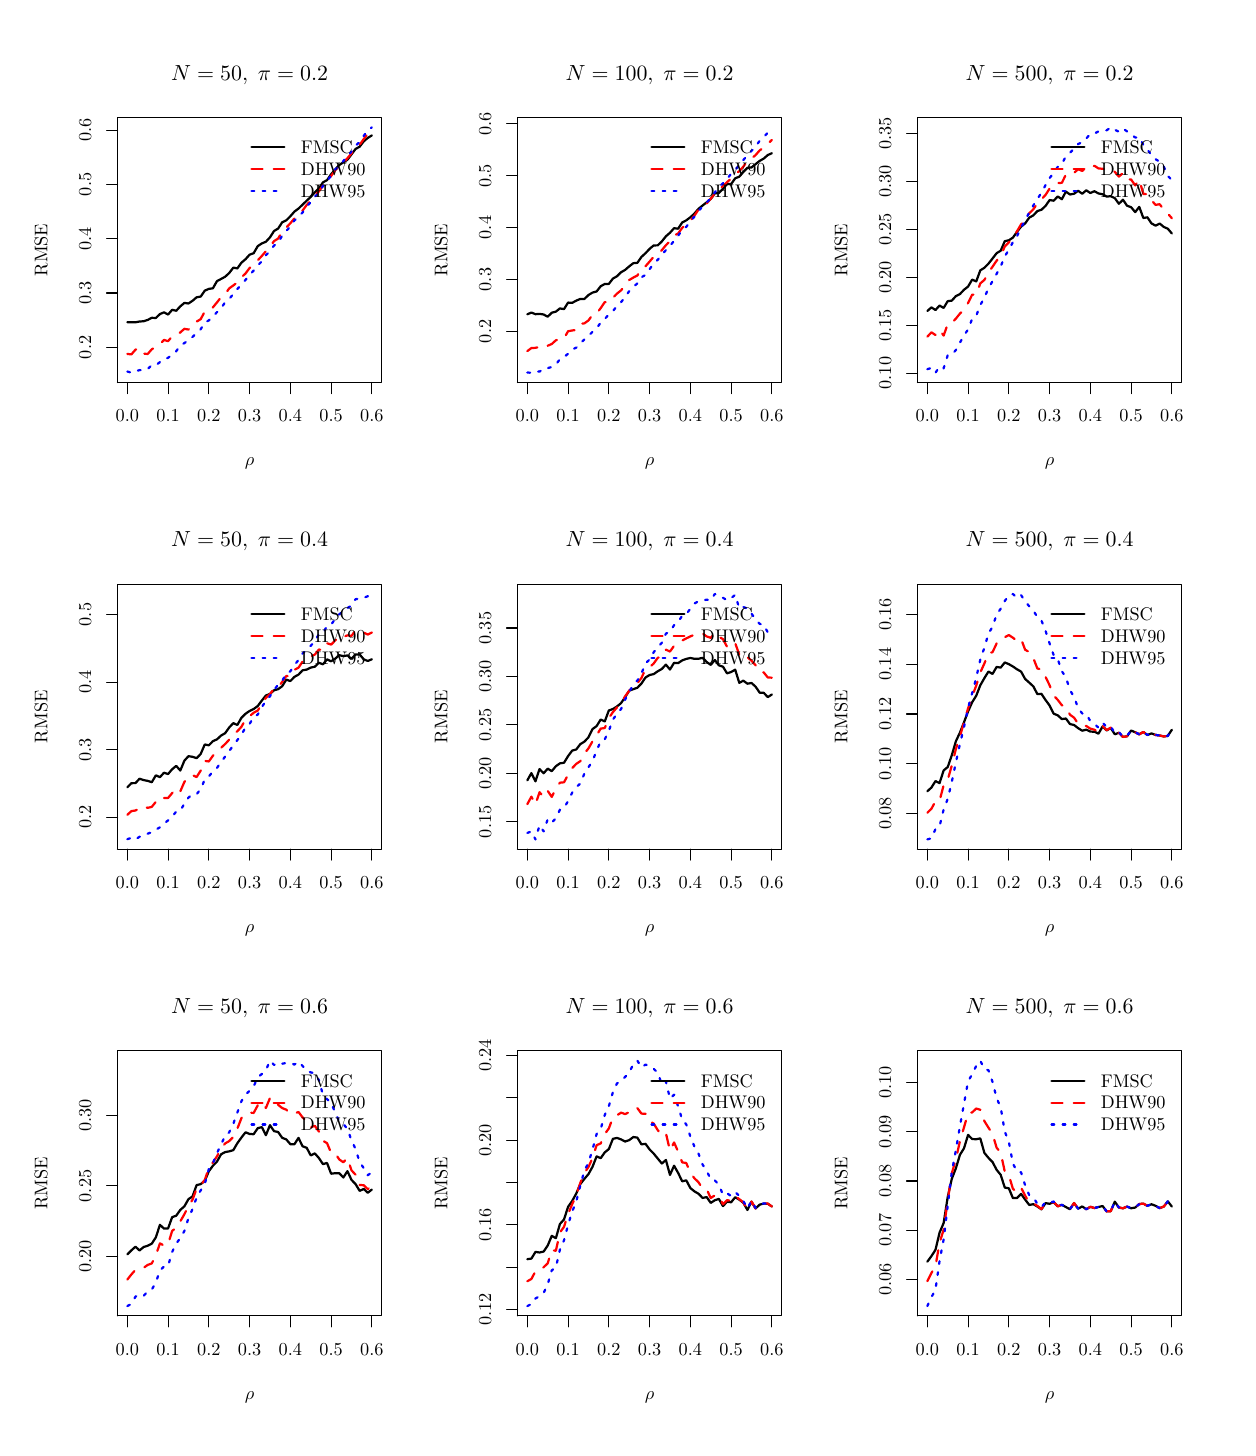
\begin{tikzpicture}[x=1pt,y=1pt]
\definecolor[named]{fillColor}{rgb}{1.00,1.00,1.00}
\path[use as bounding box,fill=fillColor,fill opacity=0.00] (0,0) rectangle (433.62,505.89);
\begin{scope}
\path[clip] ( 32.47,377.65) rectangle (127.91,473.42);
\definecolor[named]{drawColor}{rgb}{0.00,0.00,0.00}

\path[draw=drawColor,line width= 0.8pt,line join=round,line cap=round] ( 36.01,399.47) --
	( 37.48,399.47) --
	( 38.95,399.41) --
	( 40.42,399.71) --
	( 41.90,399.80) --
	( 43.37,400.28) --
	( 44.84,401.04) --
	( 46.32,400.99) --
	( 47.79,402.40) --
	( 49.26,403.03) --
	( 50.73,402.22) --
	( 52.21,403.94) --
	( 53.68,403.59) --
	( 55.15,405.19) --
	( 56.63,406.43) --
	( 58.10,406.22) --
	( 59.57,407.19) --
	( 61.04,408.46) --
	( 62.52,408.72) --
	( 63.99,410.85) --
	( 65.46,411.50) --
	( 66.93,411.71) --
	( 68.41,414.31) --
	( 69.88,415.08) --
	( 71.35,415.88) --
	( 72.83,417.24) --
	( 74.30,419.17) --
	( 75.77,418.89) --
	( 77.24,420.97) --
	( 78.72,422.22) --
	( 80.19,423.86) --
	( 81.66,424.39) --
	( 83.14,426.96) --
	( 84.61,427.92) --
	( 86.08,428.52) --
	( 87.55,430.12) --
	( 89.03,432.42) --
	( 90.50,433.29) --
	( 91.97,435.56) --
	( 93.44,436.26) --
	( 94.92,437.75) --
	( 96.39,439.42) --
	( 97.86,440.52) --
	( 99.34,441.93) --
	(100.81,443.36) --
	(102.28,444.71) --
	(103.75,446.39) --
	(105.23,447.80) --
	(106.70,450.00) --
	(108.17,450.78) --
	(109.65,452.94) --
	(111.12,454.63) --
	(112.59,456.24) --
	(114.06,457.24) --
	(115.54,458.16) --
	(117.01,460.09) --
	(118.48,462.06) --
	(119.95,462.87) --
	(121.43,464.80) --
	(122.90,466.05) --
	(124.37,466.95);
\end{scope}
\begin{scope}
\path[clip] (  0.00,  0.00) rectangle (433.62,505.89);
\definecolor[named]{drawColor}{rgb}{0.00,0.00,0.00}

\path[draw=drawColor,line width= 0.4pt,line join=round,line cap=round] ( 36.01,377.65) -- (124.37,377.65);

\path[draw=drawColor,line width= 0.4pt,line join=round,line cap=round] ( 36.01,377.65) -- ( 36.01,373.69);

\path[draw=drawColor,line width= 0.4pt,line join=round,line cap=round] ( 50.73,377.65) -- ( 50.73,373.69);

\path[draw=drawColor,line width= 0.4pt,line join=round,line cap=round] ( 65.46,377.65) -- ( 65.46,373.69);

\path[draw=drawColor,line width= 0.4pt,line join=round,line cap=round] ( 80.19,377.65) -- ( 80.19,373.69);

\path[draw=drawColor,line width= 0.4pt,line join=round,line cap=round] ( 94.92,377.65) -- ( 94.92,373.69);

\path[draw=drawColor,line width= 0.4pt,line join=round,line cap=round] (109.65,377.65) -- (109.65,373.69);

\path[draw=drawColor,line width= 0.4pt,line join=round,line cap=round] (124.37,377.65) -- (124.37,373.69);

\node[text=drawColor,anchor=base,inner sep=0pt, outer sep=0pt, scale=  0.66] at ( 36.01,363.40) {0.0};

\node[text=drawColor,anchor=base,inner sep=0pt, outer sep=0pt, scale=  0.66] at ( 50.73,363.40) {0.1};

\node[text=drawColor,anchor=base,inner sep=0pt, outer sep=0pt, scale=  0.66] at ( 65.46,363.40) {0.2};

\node[text=drawColor,anchor=base,inner sep=0pt, outer sep=0pt, scale=  0.66] at ( 80.19,363.40) {0.3};

\node[text=drawColor,anchor=base,inner sep=0pt, outer sep=0pt, scale=  0.66] at ( 94.92,363.40) {0.4};

\node[text=drawColor,anchor=base,inner sep=0pt, outer sep=0pt, scale=  0.66] at (109.65,363.40) {0.5};

\node[text=drawColor,anchor=base,inner sep=0pt, outer sep=0pt, scale=  0.66] at (124.37,363.40) {0.6};

\path[draw=drawColor,line width= 0.4pt,line join=round,line cap=round] ( 32.47,390.37) -- ( 32.47,468.88);

\path[draw=drawColor,line width= 0.4pt,line join=round,line cap=round] ( 32.47,390.37) -- ( 28.51,390.37);

\path[draw=drawColor,line width= 0.4pt,line join=round,line cap=round] ( 32.47,410.00) -- ( 28.51,410.00);

\path[draw=drawColor,line width= 0.4pt,line join=round,line cap=round] ( 32.47,429.62) -- ( 28.51,429.62);

\path[draw=drawColor,line width= 0.4pt,line join=round,line cap=round] ( 32.47,449.25) -- ( 28.51,449.25);

\path[draw=drawColor,line width= 0.4pt,line join=round,line cap=round] ( 32.47,468.88) -- ( 28.51,468.88);

\node[text=drawColor,rotate= 90.00,anchor=base,inner sep=0pt, outer sep=0pt, scale=  0.66] at ( 22.97,390.37) {0.2};

\node[text=drawColor,rotate= 90.00,anchor=base,inner sep=0pt, outer sep=0pt, scale=  0.66] at ( 22.97,410.00) {0.3};

\node[text=drawColor,rotate= 90.00,anchor=base,inner sep=0pt, outer sep=0pt, scale=  0.66] at ( 22.97,429.62) {0.4};

\node[text=drawColor,rotate= 90.00,anchor=base,inner sep=0pt, outer sep=0pt, scale=  0.66] at ( 22.97,449.25) {0.5};

\node[text=drawColor,rotate= 90.00,anchor=base,inner sep=0pt, outer sep=0pt, scale=  0.66] at ( 22.97,468.88) {0.6};

\path[draw=drawColor,line width= 0.4pt,line join=round,line cap=round] ( 32.47,377.65) --
	(127.91,377.65) --
	(127.91,473.42) --
	( 32.47,473.42) --
	( 32.47,377.65);
\end{scope}
\begin{scope}
\path[clip] (  0.00,337.26) rectangle (144.54,505.89);
\definecolor[named]{drawColor}{rgb}{0.00,0.00,0.00}

\node[text=drawColor,anchor=base,inner sep=0pt, outer sep=0pt, scale=  0.79] at ( 80.19,486.92) {\bfseries $N=50, \;\pi=0.2$};

\node[text=drawColor,anchor=base,inner sep=0pt, outer sep=0pt, scale=  0.66] at ( 80.19,347.56) {$\rho$};

\node[text=drawColor,rotate= 90.00,anchor=base,inner sep=0pt, outer sep=0pt, scale=  0.66] at (  7.13,425.53) {RMSE};
\end{scope}
\begin{scope}
\path[clip] ( 32.47,377.65) rectangle (127.91,473.42);
\definecolor[named]{drawColor}{rgb}{1.00,0.00,0.00}

\path[draw=drawColor,line width= 0.8pt,dash pattern=on 4pt off 4pt ,line join=round,line cap=round] ( 36.01,387.99) --
	( 37.48,387.83) --
	( 38.95,389.53) --
	( 40.42,390.06) --
	( 41.90,388.10) --
	( 43.37,387.97) --
	( 44.84,389.67) --
	( 46.32,390.50) --
	( 47.79,391.44) --
	( 49.26,393.07) --
	( 50.73,392.60) --
	( 52.21,394.37) --
	( 53.68,394.66) --
	( 55.15,395.77) --
	( 56.63,397.08) --
	( 58.10,396.80) --
	( 59.57,398.50) --
	( 61.04,399.68) --
	( 62.52,400.55) --
	( 63.99,403.32) --
	( 65.46,403.75) --
	( 66.93,404.82) --
	( 68.41,406.61) --
	( 69.88,408.51) --
	( 71.35,409.62) --
	( 72.83,411.69) --
	( 74.30,412.73) --
	( 75.77,413.85) --
	( 77.24,415.69) --
	( 78.72,417.06) --
	( 80.19,419.06) --
	( 81.66,420.06) --
	( 83.14,421.84) --
	( 84.61,423.39) --
	( 86.08,425.10) --
	( 87.55,426.68) --
	( 89.03,428.77) --
	( 90.50,429.68) --
	( 91.97,432.18) --
	( 93.44,433.64) --
	( 94.92,435.22) --
	( 96.39,436.96) --
	( 97.86,438.24) --
	( 99.34,439.80) --
	(100.81,441.80) --
	(102.28,443.40) --
	(103.75,445.27) --
	(105.23,446.72) --
	(106.70,448.79) --
	(108.17,450.27) --
	(109.65,452.29) --
	(111.12,454.38) --
	(112.59,455.75) --
	(114.06,457.10) --
	(115.54,458.70) --
	(117.01,460.46) --
	(118.48,462.67) --
	(119.95,463.56) --
	(121.43,465.64) --
	(122.90,467.55) --
	(124.37,468.42);
\definecolor[named]{drawColor}{rgb}{0.00,0.00,1.00}

\path[draw=drawColor,line width= 0.8pt,dash pattern=on 1pt off 3pt ,line join=round,line cap=round] ( 36.01,381.65) --
	( 37.48,381.20) --
	( 38.95,381.69) --
	( 40.42,382.15) --
	( 41.90,382.10) --
	( 43.37,382.56) --
	( 44.84,383.91) --
	( 46.32,383.88) --
	( 47.79,385.04) --
	( 49.26,386.04) --
	( 50.73,386.59) --
	( 52.21,387.72) --
	( 53.68,388.96) --
	( 55.15,391.10) --
	( 56.63,391.91) --
	( 58.10,392.95) --
	( 59.57,394.15) --
	( 61.04,395.56) --
	( 62.52,396.92) --
	( 63.99,399.31) --
	( 65.46,400.10) --
	( 66.93,401.49) --
	( 68.41,403.10) --
	( 69.88,404.49) --
	( 71.35,406.68) --
	( 72.83,407.84) --
	( 74.30,409.64) --
	( 75.77,411.46) --
	( 77.24,413.02) --
	( 78.72,414.74) --
	( 80.19,416.56) --
	( 81.66,418.11) --
	( 83.14,419.97) --
	( 84.61,421.48) --
	( 86.08,423.67) --
	( 87.55,425.15) --
	( 89.03,427.16) --
	( 90.50,428.18) --
	( 91.97,430.75) --
	( 93.44,432.41) --
	( 94.92,434.03) --
	( 96.39,436.22) --
	( 97.86,437.60) --
	( 99.34,439.08) --
	(100.81,441.24) --
	(102.28,442.83) --
	(103.75,444.80) --
	(105.23,446.18) --
	(106.70,448.66) --
	(108.17,450.46) --
	(109.65,452.40) --
	(111.12,454.59) --
	(112.59,456.17) --
	(114.06,457.68) --
	(115.54,459.45) --
	(117.01,461.12) --
	(118.48,463.24) --
	(119.95,464.57) --
	(121.43,466.80) --
	(122.90,468.74) --
	(124.37,469.87);
\definecolor[named]{drawColor}{rgb}{0.00,0.00,0.00}

\path[draw=drawColor,line width= 0.8pt,line join=round,line cap=round] ( 80.89,462.63) -- ( 92.77,462.63);
\definecolor[named]{drawColor}{rgb}{1.00,0.00,0.00}

\path[draw=drawColor,line width= 0.8pt,dash pattern=on 4pt off 4pt ,line join=round,line cap=round] ( 80.89,454.71) -- ( 92.77,454.71);
\definecolor[named]{drawColor}{rgb}{0.00,0.00,1.00}

\path[draw=drawColor,line width= 0.8pt,dash pattern=on 1pt off 3pt ,line join=round,line cap=round] ( 80.89,446.79) -- ( 92.77,446.79);
\definecolor[named]{drawColor}{rgb}{0.00,0.00,0.00}

\node[text=drawColor,anchor=base west,inner sep=0pt, outer sep=0pt, scale=  0.66] at ( 98.71,460.35) {FMSC};

\node[text=drawColor,anchor=base west,inner sep=0pt, outer sep=0pt, scale=  0.66] at ( 98.71,452.43) {DHW90};

\node[text=drawColor,anchor=base west,inner sep=0pt, outer sep=0pt, scale=  0.66] at ( 98.71,444.51) {DHW95};
\end{scope}
\begin{scope}
\path[clip] (177.01,377.65) rectangle (272.45,473.42);
\definecolor[named]{drawColor}{rgb}{0.00,0.00,0.00}

\path[draw=drawColor,line width= 0.8pt,line join=round,line cap=round] (180.55,402.31) --
	(182.02,402.94) --
	(183.49,402.35) --
	(184.96,402.47) --
	(186.44,402.24) --
	(187.91,401.44) --
	(189.38,402.89) --
	(190.86,403.28) --
	(192.33,404.44) --
	(193.80,404.18) --
	(195.27,406.55) --
	(196.75,406.44) --
	(198.22,407.25) --
	(199.69,407.86) --
	(201.17,407.85) --
	(202.64,409.28) --
	(204.11,410.16) --
	(205.58,410.57) --
	(207.06,412.45) --
	(208.53,413.28) --
	(210.00,413.30) --
	(211.47,415.21) --
	(212.95,416.07) --
	(214.42,417.51) --
	(215.89,418.36) --
	(217.37,419.64) --
	(218.84,420.78) --
	(220.31,420.91) --
	(221.78,423.04) --
	(223.26,424.40) --
	(224.73,425.97) --
	(226.20,427.19) --
	(227.68,427.23) --
	(229.15,428.64) --
	(230.62,430.50) --
	(232.09,431.77) --
	(233.57,433.43) --
	(235.04,433.24) --
	(236.51,435.50) --
	(237.98,436.26) --
	(239.46,437.37) --
	(240.93,438.72) --
	(242.40,440.44) --
	(243.88,441.62) --
	(245.35,442.77) --
	(246.82,443.98) --
	(248.29,445.98) --
	(249.77,446.13) --
	(251.24,447.68) --
	(252.71,449.35) --
	(254.19,449.38) --
	(255.66,451.45) --
	(257.13,452.04) --
	(258.60,453.74) --
	(260.08,455.26) --
	(261.55,455.37) --
	(263.02,456.57) --
	(264.50,457.74) --
	(265.97,458.58) --
	(267.44,459.86) --
	(268.91,460.52);
\end{scope}
\begin{scope}
\path[clip] (  0.00,  0.00) rectangle (433.62,505.89);
\definecolor[named]{drawColor}{rgb}{0.00,0.00,0.00}

\path[draw=drawColor,line width= 0.4pt,line join=round,line cap=round] (180.55,377.65) -- (268.91,377.65);

\path[draw=drawColor,line width= 0.4pt,line join=round,line cap=round] (180.55,377.65) -- (180.55,373.69);

\path[draw=drawColor,line width= 0.4pt,line join=round,line cap=round] (195.27,377.65) -- (195.27,373.69);

\path[draw=drawColor,line width= 0.4pt,line join=round,line cap=round] (210.00,377.65) -- (210.00,373.69);

\path[draw=drawColor,line width= 0.4pt,line join=round,line cap=round] (224.73,377.65) -- (224.73,373.69);

\path[draw=drawColor,line width= 0.4pt,line join=round,line cap=round] (239.46,377.65) -- (239.46,373.69);

\path[draw=drawColor,line width= 0.4pt,line join=round,line cap=round] (254.19,377.65) -- (254.19,373.69);

\path[draw=drawColor,line width= 0.4pt,line join=round,line cap=round] (268.91,377.65) -- (268.91,373.69);

\node[text=drawColor,anchor=base,inner sep=0pt, outer sep=0pt, scale=  0.66] at (180.55,363.40) {0.0};

\node[text=drawColor,anchor=base,inner sep=0pt, outer sep=0pt, scale=  0.66] at (195.27,363.40) {0.1};

\node[text=drawColor,anchor=base,inner sep=0pt, outer sep=0pt, scale=  0.66] at (210.00,363.40) {0.2};

\node[text=drawColor,anchor=base,inner sep=0pt, outer sep=0pt, scale=  0.66] at (224.73,363.40) {0.3};

\node[text=drawColor,anchor=base,inner sep=0pt, outer sep=0pt, scale=  0.66] at (239.46,363.40) {0.4};

\node[text=drawColor,anchor=base,inner sep=0pt, outer sep=0pt, scale=  0.66] at (254.19,363.40) {0.5};

\node[text=drawColor,anchor=base,inner sep=0pt, outer sep=0pt, scale=  0.66] at (268.91,363.40) {0.6};

\path[draw=drawColor,line width= 0.4pt,line join=round,line cap=round] (177.01,396.12) -- (177.01,471.23);

\path[draw=drawColor,line width= 0.4pt,line join=round,line cap=round] (177.01,396.12) -- (173.05,396.12);

\path[draw=drawColor,line width= 0.4pt,line join=round,line cap=round] (177.01,414.90) -- (173.05,414.90);

\path[draw=drawColor,line width= 0.4pt,line join=round,line cap=round] (177.01,433.68) -- (173.05,433.68);

\path[draw=drawColor,line width= 0.4pt,line join=round,line cap=round] (177.01,452.45) -- (173.05,452.45);

\path[draw=drawColor,line width= 0.4pt,line join=round,line cap=round] (177.01,471.23) -- (173.05,471.23);

\node[text=drawColor,rotate= 90.00,anchor=base,inner sep=0pt, outer sep=0pt, scale=  0.66] at (167.51,396.12) {0.2};

\node[text=drawColor,rotate= 90.00,anchor=base,inner sep=0pt, outer sep=0pt, scale=  0.66] at (167.51,414.90) {0.3};

\node[text=drawColor,rotate= 90.00,anchor=base,inner sep=0pt, outer sep=0pt, scale=  0.66] at (167.51,433.68) {0.4};

\node[text=drawColor,rotate= 90.00,anchor=base,inner sep=0pt, outer sep=0pt, scale=  0.66] at (167.51,452.45) {0.5};

\node[text=drawColor,rotate= 90.00,anchor=base,inner sep=0pt, outer sep=0pt, scale=  0.66] at (167.51,471.23) {0.6};

\path[draw=drawColor,line width= 0.4pt,line join=round,line cap=round] (177.01,377.65) --
	(272.45,377.65) --
	(272.45,473.42) --
	(177.01,473.42) --
	(177.01,377.65);
\end{scope}
\begin{scope}
\path[clip] (144.54,337.26) rectangle (289.08,505.89);
\definecolor[named]{drawColor}{rgb}{0.00,0.00,0.00}

\node[text=drawColor,anchor=base,inner sep=0pt, outer sep=0pt, scale=  0.79] at (224.73,486.92) {\bfseries $N=100, \;\pi=0.2$};

\node[text=drawColor,anchor=base,inner sep=0pt, outer sep=0pt, scale=  0.66] at (224.73,347.56) {$\rho$};

\node[text=drawColor,rotate= 90.00,anchor=base,inner sep=0pt, outer sep=0pt, scale=  0.66] at (151.67,425.53) {RMSE};
\end{scope}
\begin{scope}
\path[clip] (177.01,377.65) rectangle (272.45,473.42);
\definecolor[named]{drawColor}{rgb}{1.00,0.00,0.00}

\path[draw=drawColor,line width= 0.8pt,dash pattern=on 4pt off 4pt ,line join=round,line cap=round] (180.55,389.02) --
	(182.02,390.11) --
	(183.49,390.20) --
	(184.96,390.54) --
	(186.44,391.36) --
	(187.91,390.96) --
	(189.38,391.58) --
	(190.86,392.92) --
	(192.33,393.32) --
	(193.80,393.59) --
	(195.27,396.19) --
	(196.75,396.47) --
	(198.22,396.65) --
	(199.69,398.85) --
	(201.17,399.04) --
	(202.64,400.10) --
	(204.11,402.13) --
	(205.58,402.58) --
	(207.06,404.56) --
	(208.53,406.72) --
	(210.00,406.69) --
	(211.47,408.25) --
	(212.95,409.80) --
	(214.42,410.96) --
	(215.89,412.83) --
	(217.37,414.70) --
	(218.84,415.58) --
	(220.31,416.33) --
	(221.78,418.73) --
	(223.26,419.68) --
	(224.73,421.37) --
	(226.20,423.09) --
	(227.68,424.07) --
	(229.15,425.47) --
	(230.62,427.28) --
	(232.09,428.78) --
	(233.57,430.79) --
	(235.04,431.50) --
	(236.51,433.54) --
	(237.98,434.84) --
	(239.46,436.17) --
	(240.93,437.95) --
	(242.40,440.14) --
	(243.88,441.26) --
	(245.35,442.37) --
	(246.82,444.09) --
	(248.29,445.89) --
	(249.77,447.31) --
	(251.24,448.68) --
	(252.71,450.07) --
	(254.19,451.33) --
	(255.66,452.91) --
	(257.13,454.05) --
	(258.60,455.67) --
	(260.08,457.75) --
	(261.55,458.56) --
	(263.02,459.84) --
	(264.50,461.53) --
	(265.97,462.59) --
	(267.44,463.93) --
	(268.91,465.31);
\definecolor[named]{drawColor}{rgb}{0.00,0.00,1.00}

\path[draw=drawColor,line width= 0.8pt,dash pattern=on 1pt off 3pt ,line join=round,line cap=round] (180.55,381.26) --
	(182.02,381.20) --
	(183.49,381.72) --
	(184.96,381.59) --
	(186.44,382.70) --
	(187.91,382.87) --
	(189.38,383.27) --
	(190.86,384.13) --
	(192.33,386.13) --
	(193.80,386.83) --
	(195.27,388.07) --
	(196.75,389.59) --
	(198.22,390.27) --
	(199.69,391.88) --
	(201.17,393.21) --
	(202.64,394.54) --
	(204.11,395.96) --
	(205.58,397.23) --
	(207.06,399.31) --
	(208.53,400.59) --
	(210.00,402.31) --
	(211.47,403.46) --
	(212.95,405.32) --
	(214.42,406.68) --
	(215.89,408.60) --
	(217.37,410.69) --
	(218.84,412.22) --
	(220.31,413.48) --
	(221.78,415.70) --
	(223.26,416.54) --
	(224.73,418.61) --
	(226.20,420.63) --
	(227.68,422.01) --
	(229.15,423.87) --
	(230.62,425.48) --
	(232.09,427.04) --
	(233.57,428.86) --
	(235.04,430.73) --
	(236.51,432.72) --
	(237.98,433.92) --
	(239.46,435.87) --
	(240.93,437.61) --
	(242.40,439.65) --
	(243.88,441.18) --
	(245.35,442.70) --
	(246.82,444.33) --
	(248.29,446.37) --
	(249.77,448.22) --
	(251.24,449.65) --
	(252.71,451.22) --
	(254.19,453.10) --
	(255.66,454.57) --
	(257.13,456.19) --
	(258.60,458.05) --
	(260.08,459.82) --
	(261.55,461.36) --
	(263.02,462.93) --
	(264.50,465.01) --
	(265.97,466.30) --
	(267.44,467.97) --
	(268.91,469.87);
\definecolor[named]{drawColor}{rgb}{0.00,0.00,0.00}

\path[draw=drawColor,line width= 0.8pt,line join=round,line cap=round] (225.43,462.63) -- (237.31,462.63);
\definecolor[named]{drawColor}{rgb}{1.00,0.00,0.00}

\path[draw=drawColor,line width= 0.8pt,dash pattern=on 4pt off 4pt ,line join=round,line cap=round] (225.43,454.71) -- (237.31,454.71);
\definecolor[named]{drawColor}{rgb}{0.00,0.00,1.00}

\path[draw=drawColor,line width= 0.8pt,dash pattern=on 1pt off 3pt ,line join=round,line cap=round] (225.43,446.79) -- (237.31,446.79);
\definecolor[named]{drawColor}{rgb}{0.00,0.00,0.00}

\node[text=drawColor,anchor=base west,inner sep=0pt, outer sep=0pt, scale=  0.66] at (243.25,460.35) {FMSC};

\node[text=drawColor,anchor=base west,inner sep=0pt, outer sep=0pt, scale=  0.66] at (243.25,452.43) {DHW90};

\node[text=drawColor,anchor=base west,inner sep=0pt, outer sep=0pt, scale=  0.66] at (243.25,444.51) {DHW95};
\end{scope}
\begin{scope}
\path[clip] (321.55,377.65) rectangle (416.99,473.42);
\definecolor[named]{drawColor}{rgb}{0.00,0.00,0.00}

\path[draw=drawColor,line width= 0.8pt,line join=round,line cap=round] (325.09,403.51) --
	(326.56,404.81) --
	(328.03,403.86) --
	(329.50,405.48) --
	(330.98,404.61) --
	(332.45,407.06) --
	(333.92,407.25) --
	(335.40,408.88) --
	(336.87,409.63) --
	(338.34,411.18) --
	(339.81,412.34) --
	(341.29,414.85) --
	(342.76,414.20) --
	(344.23,418.20) --
	(345.71,419.12) --
	(347.18,420.62) --
	(348.65,422.48) --
	(350.12,424.39) --
	(351.60,425.29) --
	(353.07,428.74) --
	(354.54,429.06) --
	(356.01,430.03) --
	(357.49,432.10) --
	(358.96,433.99) --
	(360.43,435.15) --
	(361.91,437.24) --
	(363.38,438.05) --
	(364.85,439.62) --
	(366.32,440.09) --
	(367.80,441.47) --
	(369.27,443.60) --
	(370.74,443.36) --
	(372.22,444.89) --
	(373.69,443.89) --
	(375.16,446.65) --
	(376.63,445.61) --
	(378.11,445.87) --
	(379.58,446.95) --
	(381.05,445.87) --
	(382.52,447.12) --
	(384.00,446.14) --
	(385.47,446.79) --
	(386.94,445.97) --
	(388.42,445.69) --
	(389.89,444.85) --
	(391.36,444.99) --
	(392.83,444.29) --
	(394.31,442.25) --
	(395.78,443.71) --
	(397.25,441.55) --
	(398.73,441.01) --
	(400.20,439.23) --
	(401.67,441.12) --
	(403.14,437.11) --
	(404.62,437.36) --
	(406.09,435.16) --
	(407.56,434.34) --
	(409.04,435.11) --
	(410.51,433.89) --
	(411.98,433.24) --
	(413.45,431.52);
\end{scope}
\begin{scope}
\path[clip] (  0.00,  0.00) rectangle (433.62,505.89);
\definecolor[named]{drawColor}{rgb}{0.00,0.00,0.00}

\path[draw=drawColor,line width= 0.4pt,line join=round,line cap=round] (325.09,377.65) -- (413.45,377.65);

\path[draw=drawColor,line width= 0.4pt,line join=round,line cap=round] (325.09,377.65) -- (325.09,373.69);

\path[draw=drawColor,line width= 0.4pt,line join=round,line cap=round] (339.81,377.65) -- (339.81,373.69);

\path[draw=drawColor,line width= 0.4pt,line join=round,line cap=round] (354.54,377.65) -- (354.54,373.69);

\path[draw=drawColor,line width= 0.4pt,line join=round,line cap=round] (369.27,377.65) -- (369.27,373.69);

\path[draw=drawColor,line width= 0.4pt,line join=round,line cap=round] (384.00,377.65) -- (384.00,373.69);

\path[draw=drawColor,line width= 0.4pt,line join=round,line cap=round] (398.73,377.65) -- (398.73,373.69);

\path[draw=drawColor,line width= 0.4pt,line join=round,line cap=round] (413.45,377.65) -- (413.45,373.69);

\node[text=drawColor,anchor=base,inner sep=0pt, outer sep=0pt, scale=  0.66] at (325.09,363.40) {0.0};

\node[text=drawColor,anchor=base,inner sep=0pt, outer sep=0pt, scale=  0.66] at (339.81,363.40) {0.1};

\node[text=drawColor,anchor=base,inner sep=0pt, outer sep=0pt, scale=  0.66] at (354.54,363.40) {0.2};

\node[text=drawColor,anchor=base,inner sep=0pt, outer sep=0pt, scale=  0.66] at (369.27,363.40) {0.3};

\node[text=drawColor,anchor=base,inner sep=0pt, outer sep=0pt, scale=  0.66] at (384.00,363.40) {0.4};

\node[text=drawColor,anchor=base,inner sep=0pt, outer sep=0pt, scale=  0.66] at (398.73,363.40) {0.5};

\node[text=drawColor,anchor=base,inner sep=0pt, outer sep=0pt, scale=  0.66] at (413.45,363.40) {0.6};

\path[draw=drawColor,line width= 0.4pt,line join=round,line cap=round] (321.55,381.08) -- (321.55,467.59);

\path[draw=drawColor,line width= 0.4pt,line join=round,line cap=round] (321.55,381.08) -- (317.59,381.08);

\path[draw=drawColor,line width= 0.4pt,line join=round,line cap=round] (321.55,398.38) -- (317.59,398.38);

\path[draw=drawColor,line width= 0.4pt,line join=round,line cap=round] (321.55,415.68) -- (317.59,415.68);

\path[draw=drawColor,line width= 0.4pt,line join=round,line cap=round] (321.55,432.99) -- (317.59,432.99);

\path[draw=drawColor,line width= 0.4pt,line join=round,line cap=round] (321.55,450.29) -- (317.59,450.29);

\path[draw=drawColor,line width= 0.4pt,line join=round,line cap=round] (321.55,467.59) -- (317.59,467.59);

\node[text=drawColor,rotate= 90.00,anchor=base,inner sep=0pt, outer sep=0pt, scale=  0.66] at (312.05,381.08) {0.10};

\node[text=drawColor,rotate= 90.00,anchor=base,inner sep=0pt, outer sep=0pt, scale=  0.66] at (312.05,398.38) {0.15};

\node[text=drawColor,rotate= 90.00,anchor=base,inner sep=0pt, outer sep=0pt, scale=  0.66] at (312.05,415.68) {0.20};

\node[text=drawColor,rotate= 90.00,anchor=base,inner sep=0pt, outer sep=0pt, scale=  0.66] at (312.05,432.99) {0.25};

\node[text=drawColor,rotate= 90.00,anchor=base,inner sep=0pt, outer sep=0pt, scale=  0.66] at (312.05,450.29) {0.30};

\node[text=drawColor,rotate= 90.00,anchor=base,inner sep=0pt, outer sep=0pt, scale=  0.66] at (312.05,467.59) {0.35};

\path[draw=drawColor,line width= 0.4pt,line join=round,line cap=round] (321.55,377.65) --
	(416.99,377.65) --
	(416.99,473.42) --
	(321.55,473.42) --
	(321.55,377.65);
\end{scope}
\begin{scope}
\path[clip] (289.08,337.26) rectangle (433.62,505.89);
\definecolor[named]{drawColor}{rgb}{0.00,0.00,0.00}

\node[text=drawColor,anchor=base,inner sep=0pt, outer sep=0pt, scale=  0.79] at (369.27,486.92) {\bfseries $N=500, \;\pi=0.2$};

\node[text=drawColor,anchor=base,inner sep=0pt, outer sep=0pt, scale=  0.66] at (369.27,347.56) {$\rho$};

\node[text=drawColor,rotate= 90.00,anchor=base,inner sep=0pt, outer sep=0pt, scale=  0.66] at (296.21,425.53) {RMSE};
\end{scope}
\begin{scope}
\path[clip] (321.55,377.65) rectangle (416.99,473.42);
\definecolor[named]{drawColor}{rgb}{1.00,0.00,0.00}

\path[draw=drawColor,line width= 0.8pt,dash pattern=on 4pt off 4pt ,line join=round,line cap=round] (325.09,394.22) --
	(326.56,395.79) --
	(328.03,394.84) --
	(329.50,396.74) --
	(330.98,394.62) --
	(332.45,398.76) --
	(333.92,399.16) --
	(335.40,400.75) --
	(336.87,402.58) --
	(338.34,403.92) --
	(339.81,406.42) --
	(341.29,409.41) --
	(342.76,409.39) --
	(344.23,413.48) --
	(345.71,414.75) --
	(347.18,417.39) --
	(348.65,419.51) --
	(350.12,421.67) --
	(351.60,423.45) --
	(353.07,426.82) --
	(354.54,428.31) --
	(356.01,429.95) --
	(357.49,432.30) --
	(358.96,434.81) --
	(360.43,436.46) --
	(361.91,438.81) --
	(363.38,440.24) --
	(364.85,442.36) --
	(366.32,443.87) --
	(367.80,445.44) --
	(369.27,447.74) --
	(370.74,448.50) --
	(372.22,449.78) --
	(373.69,449.80) --
	(375.16,452.79) --
	(376.63,452.56) --
	(378.11,453.43) --
	(379.58,454.73) --
	(381.05,454.12) --
	(382.52,455.24) --
	(384.00,455.25) --
	(385.47,455.97) --
	(386.94,455.02) --
	(388.42,454.89) --
	(389.89,454.66) --
	(391.36,454.74) --
	(392.83,453.77) --
	(394.31,452.06) --
	(395.78,453.37) --
	(397.25,451.20) --
	(398.73,451.00) --
	(400.20,448.88) --
	(401.67,450.95) --
	(403.14,445.80) --
	(404.62,445.70) --
	(406.09,443.53) --
	(407.56,441.84) --
	(409.04,442.10) --
	(410.51,440.10) --
	(411.98,438.72) --
	(413.45,437.02);
\definecolor[named]{drawColor}{rgb}{0.00,0.00,1.00}

\path[draw=drawColor,line width= 0.8pt,dash pattern=on 1pt off 3pt ,line join=round,line cap=round] (325.09,382.47) --
	(326.56,382.95) --
	(328.03,381.20) --
	(329.50,383.42) --
	(330.98,382.79) --
	(332.45,387.50) --
	(333.92,387.66) --
	(335.40,389.41) --
	(336.87,392.06) --
	(338.34,394.69) --
	(339.81,396.84) --
	(341.29,400.68) --
	(342.76,401.78) --
	(344.23,405.67) --
	(345.71,408.28) --
	(347.18,411.79) --
	(348.65,414.27) --
	(350.12,416.93) --
	(351.60,419.62) --
	(353.07,423.30) --
	(354.54,425.55) --
	(356.01,428.39) --
	(357.49,430.49) --
	(358.96,433.62) --
	(360.43,436.19) --
	(361.91,439.08) --
	(363.38,441.65) --
	(364.85,443.90) --
	(366.32,446.28) --
	(367.80,448.99) --
	(369.27,451.53) --
	(370.74,453.40) --
	(372.22,455.59) --
	(373.69,456.62) --
	(375.16,459.41) --
	(376.63,460.66) --
	(378.11,462.19) --
	(379.58,463.84) --
	(381.05,464.51) --
	(382.52,465.83) --
	(384.00,467.52) --
	(385.47,467.62) --
	(386.94,468.43) --
	(388.42,468.50) --
	(389.89,468.80) --
	(391.36,469.87) --
	(392.83,468.98) --
	(394.31,468.29) --
	(395.78,469.43) --
	(397.25,468.41) --
	(398.73,467.29) --
	(400.20,466.22) --
	(401.67,466.20) --
	(403.14,463.61) --
	(404.62,461.86) --
	(406.09,459.76) --
	(407.56,458.37) --
	(409.04,457.42) --
	(410.51,455.71) --
	(411.98,452.35) --
	(413.45,450.81);
\definecolor[named]{drawColor}{rgb}{0.00,0.00,0.00}

\path[draw=drawColor,line width= 0.8pt,line join=round,line cap=round] (369.97,462.63) -- (381.85,462.63);
\definecolor[named]{drawColor}{rgb}{1.00,0.00,0.00}

\path[draw=drawColor,line width= 0.8pt,dash pattern=on 4pt off 4pt ,line join=round,line cap=round] (369.97,454.71) -- (381.85,454.71);
\definecolor[named]{drawColor}{rgb}{0.00,0.00,1.00}

\path[draw=drawColor,line width= 0.8pt,dash pattern=on 1pt off 3pt ,line join=round,line cap=round] (369.97,446.79) -- (381.85,446.79);
\definecolor[named]{drawColor}{rgb}{0.00,0.00,0.00}

\node[text=drawColor,anchor=base west,inner sep=0pt, outer sep=0pt, scale=  0.66] at (387.79,460.35) {FMSC};

\node[text=drawColor,anchor=base west,inner sep=0pt, outer sep=0pt, scale=  0.66] at (387.79,452.43) {DHW90};

\node[text=drawColor,anchor=base west,inner sep=0pt, outer sep=0pt, scale=  0.66] at (387.79,444.51) {DHW95};
\end{scope}
\begin{scope}
\path[clip] ( 32.47,209.02) rectangle (127.91,304.79);
\definecolor[named]{drawColor}{rgb}{0.00,0.00,0.00}

\path[draw=drawColor,line width= 0.8pt,line join=round,line cap=round] ( 36.01,231.39) --
	( 37.48,232.89) --
	( 38.95,232.91) --
	( 40.42,234.50) --
	( 41.90,234.01) --
	( 43.37,233.72) --
	( 44.84,233.22) --
	( 46.32,235.72) --
	( 47.79,235.06) --
	( 49.26,236.66) --
	( 50.73,236.19) --
	( 52.21,237.93) --
	( 53.68,239.14) --
	( 55.15,237.45) --
	( 56.63,241.02) --
	( 58.10,242.64) --
	( 59.57,242.42) --
	( 61.04,241.92) --
	( 62.52,243.44) --
	( 63.99,246.87) --
	( 65.46,246.56) --
	( 66.93,248.07) --
	( 68.41,248.73) --
	( 69.88,250.09) --
	( 71.35,250.94) --
	( 72.83,253.02) --
	( 74.30,254.58) --
	( 75.77,253.92) --
	( 77.24,256.52) --
	( 78.72,257.97) --
	( 80.19,258.98) --
	( 81.66,259.68) --
	( 83.14,260.77) --
	( 84.61,262.74) --
	( 86.08,264.57) --
	( 87.55,265.13) --
	( 89.03,266.46) --
	( 90.50,266.85) --
	( 91.97,267.92) --
	( 93.44,270.30) --
	( 94.92,269.78) --
	( 96.39,271.31) --
	( 97.86,272.11) --
	( 99.34,273.67) --
	(100.81,273.92) --
	(102.28,274.65) --
	(103.75,274.96) --
	(105.23,276.39) --
	(106.70,275.83) --
	(108.17,277.62) --
	(109.65,276.93) --
	(111.12,277.88) --
	(112.59,279.14) --
	(114.06,278.79) --
	(115.54,279.04) --
	(117.01,277.80) --
	(118.48,279.41) --
	(119.95,279.41) --
	(121.43,277.63) --
	(122.90,277.05) --
	(124.37,277.66);
\end{scope}
\begin{scope}
\path[clip] (  0.00,  0.00) rectangle (433.62,505.89);
\definecolor[named]{drawColor}{rgb}{0.00,0.00,0.00}

\path[draw=drawColor,line width= 0.4pt,line join=round,line cap=round] ( 36.01,209.02) -- (124.37,209.02);

\path[draw=drawColor,line width= 0.4pt,line join=round,line cap=round] ( 36.01,209.02) -- ( 36.01,205.06);

\path[draw=drawColor,line width= 0.4pt,line join=round,line cap=round] ( 50.73,209.02) -- ( 50.73,205.06);

\path[draw=drawColor,line width= 0.4pt,line join=round,line cap=round] ( 65.46,209.02) -- ( 65.46,205.06);

\path[draw=drawColor,line width= 0.4pt,line join=round,line cap=round] ( 80.19,209.02) -- ( 80.19,205.06);

\path[draw=drawColor,line width= 0.4pt,line join=round,line cap=round] ( 94.92,209.02) -- ( 94.92,205.06);

\path[draw=drawColor,line width= 0.4pt,line join=round,line cap=round] (109.65,209.02) -- (109.65,205.06);

\path[draw=drawColor,line width= 0.4pt,line join=round,line cap=round] (124.37,209.02) -- (124.37,205.06);

\node[text=drawColor,anchor=base,inner sep=0pt, outer sep=0pt, scale=  0.66] at ( 36.01,194.77) {0.0};

\node[text=drawColor,anchor=base,inner sep=0pt, outer sep=0pt, scale=  0.66] at ( 50.73,194.77) {0.1};

\node[text=drawColor,anchor=base,inner sep=0pt, outer sep=0pt, scale=  0.66] at ( 65.46,194.77) {0.2};

\node[text=drawColor,anchor=base,inner sep=0pt, outer sep=0pt, scale=  0.66] at ( 80.19,194.77) {0.3};

\node[text=drawColor,anchor=base,inner sep=0pt, outer sep=0pt, scale=  0.66] at ( 94.92,194.77) {0.4};

\node[text=drawColor,anchor=base,inner sep=0pt, outer sep=0pt, scale=  0.66] at (109.65,194.77) {0.5};

\node[text=drawColor,anchor=base,inner sep=0pt, outer sep=0pt, scale=  0.66] at (124.37,194.77) {0.6};

\path[draw=drawColor,line width= 0.4pt,line join=round,line cap=round] ( 32.47,220.56) -- ( 32.47,293.85);

\path[draw=drawColor,line width= 0.4pt,line join=round,line cap=round] ( 32.47,220.56) -- ( 28.51,220.56);

\path[draw=drawColor,line width= 0.4pt,line join=round,line cap=round] ( 32.47,244.99) -- ( 28.51,244.99);

\path[draw=drawColor,line width= 0.4pt,line join=round,line cap=round] ( 32.47,269.42) -- ( 28.51,269.42);

\path[draw=drawColor,line width= 0.4pt,line join=round,line cap=round] ( 32.47,293.85) -- ( 28.51,293.85);

\node[text=drawColor,rotate= 90.00,anchor=base,inner sep=0pt, outer sep=0pt, scale=  0.66] at ( 22.97,220.56) {0.2};

\node[text=drawColor,rotate= 90.00,anchor=base,inner sep=0pt, outer sep=0pt, scale=  0.66] at ( 22.97,244.99) {0.3};

\node[text=drawColor,rotate= 90.00,anchor=base,inner sep=0pt, outer sep=0pt, scale=  0.66] at ( 22.97,269.42) {0.4};

\node[text=drawColor,rotate= 90.00,anchor=base,inner sep=0pt, outer sep=0pt, scale=  0.66] at ( 22.97,293.85) {0.5};

\path[draw=drawColor,line width= 0.4pt,line join=round,line cap=round] ( 32.47,209.02) --
	(127.91,209.02) --
	(127.91,304.79) --
	( 32.47,304.79) --
	( 32.47,209.02);
\end{scope}
\begin{scope}
\path[clip] (  0.00,168.63) rectangle (144.54,337.26);
\definecolor[named]{drawColor}{rgb}{0.00,0.00,0.00}

\node[text=drawColor,anchor=base,inner sep=0pt, outer sep=0pt, scale=  0.79] at ( 80.19,318.29) {\bfseries $N=50, \;\pi=0.4$};

\node[text=drawColor,anchor=base,inner sep=0pt, outer sep=0pt, scale=  0.66] at ( 80.19,178.93) {$\rho$};

\node[text=drawColor,rotate= 90.00,anchor=base,inner sep=0pt, outer sep=0pt, scale=  0.66] at (  7.13,256.90) {RMSE};
\end{scope}
\begin{scope}
\path[clip] ( 32.47,209.02) rectangle (127.91,304.79);
\definecolor[named]{drawColor}{rgb}{1.00,0.00,0.00}

\path[draw=drawColor,line width= 0.8pt,dash pattern=on 4pt off 4pt ,line join=round,line cap=round] ( 36.01,221.45) --
	( 37.48,222.79) --
	( 38.95,223.02) --
	( 40.42,223.80) --
	( 41.90,224.53) --
	( 43.37,223.97) --
	( 44.84,224.32) --
	( 46.32,226.16) --
	( 47.79,225.85) --
	( 49.26,227.56) --
	( 50.73,227.54) --
	( 52.21,229.31) --
	( 53.68,231.07) --
	( 55.15,229.93) --
	( 56.63,233.35) --
	( 58.10,235.00) --
	( 59.57,235.80) --
	( 61.04,235.10) --
	( 62.52,237.43) --
	( 63.99,240.93) --
	( 65.46,240.74) --
	( 66.93,242.79) --
	( 68.41,244.11) --
	( 69.88,245.68) --
	( 71.35,247.02) --
	( 72.83,248.62) --
	( 74.30,250.73) --
	( 75.77,251.64) --
	( 77.24,253.27) --
	( 78.72,255.90) --
	( 80.19,257.06) --
	( 81.66,258.35) --
	( 83.14,259.13) --
	( 84.61,261.47) --
	( 86.08,263.73) --
	( 87.55,265.12) --
	( 89.03,267.03) --
	( 90.50,267.58) --
	( 91.97,269.48) --
	( 93.44,271.61) --
	( 94.92,271.52) --
	( 96.39,273.85) --
	( 97.86,274.61) --
	( 99.34,276.86) --
	(100.81,277.68) --
	(102.28,278.64) --
	(103.75,279.34) --
	(105.23,281.19) --
	(106.70,280.95) --
	(108.17,283.45) --
	(109.65,282.95) --
	(111.12,284.46) --
	(112.59,286.01) --
	(114.06,285.73) --
	(115.54,286.31) --
	(117.01,286.09) --
	(118.48,288.17) --
	(119.95,287.86) --
	(121.43,287.28) --
	(122.90,286.60) --
	(124.37,287.34);
\definecolor[named]{drawColor}{rgb}{0.00,0.00,1.00}

\path[draw=drawColor,line width= 0.8pt,dash pattern=on 1pt off 3pt ,line join=round,line cap=round] ( 36.01,212.65) --
	( 37.48,213.12) --
	( 38.95,212.57) --
	( 40.42,213.52) --
	( 41.90,213.86) --
	( 43.37,214.62) --
	( 44.84,215.22) --
	( 46.32,216.11) --
	( 47.79,216.93) --
	( 49.26,218.31) --
	( 50.73,219.43) --
	( 52.21,220.80) --
	( 53.68,222.63) --
	( 55.15,222.93) --
	( 56.63,225.49) --
	( 58.10,227.67) --
	( 59.57,228.90) --
	( 61.04,228.95) --
	( 62.52,230.62) --
	( 63.99,234.28) --
	( 65.46,235.34) --
	( 66.93,237.10) --
	( 68.41,238.41) --
	( 69.88,240.54) --
	( 71.35,242.50) --
	( 72.83,244.45) --
	( 74.30,246.59) --
	( 75.77,248.46) --
	( 77.24,250.39) --
	( 78.72,253.04) --
	( 80.19,254.31) --
	( 81.66,256.75) --
	( 83.14,257.67) --
	( 84.61,260.33) --
	( 86.08,262.67) --
	( 87.55,264.27) --
	( 89.03,266.63) --
	( 90.50,268.43) --
	( 91.97,269.86) --
	( 93.44,272.53) --
	( 94.92,273.30) --
	( 96.39,275.59) --
	( 97.86,277.38) --
	( 99.34,279.75) --
	(100.81,281.03) --
	(102.28,282.53) --
	(103.75,284.18) --
	(105.23,286.74) --
	(106.70,287.07) --
	(108.17,289.70) --
	(109.65,290.19) --
	(111.12,292.23) --
	(112.59,293.91) --
	(114.06,295.06) --
	(115.54,296.20) --
	(117.01,297.02) --
	(118.48,299.36) --
	(119.95,299.60) --
	(121.43,299.88) --
	(122.90,300.44) --
	(124.37,301.24);
\definecolor[named]{drawColor}{rgb}{0.00,0.00,0.00}

\path[draw=drawColor,line width= 0.8pt,line join=round,line cap=round] ( 80.89,294.00) -- ( 92.77,294.00);
\definecolor[named]{drawColor}{rgb}{1.00,0.00,0.00}

\path[draw=drawColor,line width= 0.8pt,dash pattern=on 4pt off 4pt ,line join=round,line cap=round] ( 80.89,286.08) -- ( 92.77,286.08);
\definecolor[named]{drawColor}{rgb}{0.00,0.00,1.00}

\path[draw=drawColor,line width= 0.8pt,dash pattern=on 1pt off 3pt ,line join=round,line cap=round] ( 80.89,278.16) -- ( 92.77,278.16);
\definecolor[named]{drawColor}{rgb}{0.00,0.00,0.00}

\node[text=drawColor,anchor=base west,inner sep=0pt, outer sep=0pt, scale=  0.66] at ( 98.71,291.72) {FMSC};

\node[text=drawColor,anchor=base west,inner sep=0pt, outer sep=0pt, scale=  0.66] at ( 98.71,283.80) {DHW90};

\node[text=drawColor,anchor=base west,inner sep=0pt, outer sep=0pt, scale=  0.66] at ( 98.71,275.88) {DHW95};
\end{scope}
\begin{scope}
\path[clip] (177.01,209.02) rectangle (272.45,304.79);
\definecolor[named]{drawColor}{rgb}{0.00,0.00,0.00}

\path[draw=drawColor,line width= 0.8pt,line join=round,line cap=round] (180.55,233.92) --
	(182.02,236.53) --
	(183.49,233.55) --
	(184.96,237.98) --
	(186.44,236.46) --
	(187.91,238.14) --
	(189.38,237.23) --
	(190.86,239.02) --
	(192.33,240.05) --
	(193.80,240.26) --
	(195.27,242.67) --
	(196.75,244.65) --
	(198.22,245.07) --
	(199.69,246.99) --
	(201.17,247.89) --
	(202.64,249.46) --
	(204.11,252.44) --
	(205.58,253.51) --
	(207.06,255.89) --
	(208.53,255.19) --
	(210.00,259.18) --
	(211.47,259.68) --
	(212.95,260.60) --
	(214.42,261.82) --
	(215.89,263.98) --
	(217.37,266.31) --
	(218.84,266.85) --
	(220.31,267.37) --
	(221.78,268.90) --
	(223.26,271.08) --
	(224.73,271.97) --
	(226.20,272.30) --
	(227.68,273.32) --
	(229.15,274.16) --
	(230.62,275.73) --
	(232.09,273.95) --
	(233.57,276.37) --
	(235.04,276.28) --
	(236.51,277.26) --
	(237.98,277.79) --
	(239.46,278.13) --
	(240.93,277.82) --
	(242.40,277.84) --
	(243.88,278.18) --
	(245.35,276.67) --
	(246.82,275.62) --
	(248.29,277.40) --
	(249.77,275.46) --
	(251.24,274.99) --
	(252.71,272.57) --
	(254.19,273.06) --
	(255.66,273.90) --
	(257.13,269.14) --
	(258.60,269.93) --
	(260.08,268.83) --
	(261.55,269.09) --
	(263.02,267.77) --
	(264.50,265.60) --
	(265.97,265.55) --
	(267.44,263.98) --
	(268.91,264.94);
\end{scope}
\begin{scope}
\path[clip] (  0.00,  0.00) rectangle (433.62,505.89);
\definecolor[named]{drawColor}{rgb}{0.00,0.00,0.00}

\path[draw=drawColor,line width= 0.4pt,line join=round,line cap=round] (180.55,209.02) -- (268.91,209.02);

\path[draw=drawColor,line width= 0.4pt,line join=round,line cap=round] (180.55,209.02) -- (180.55,205.06);

\path[draw=drawColor,line width= 0.4pt,line join=round,line cap=round] (195.27,209.02) -- (195.27,205.06);

\path[draw=drawColor,line width= 0.4pt,line join=round,line cap=round] (210.00,209.02) -- (210.00,205.06);

\path[draw=drawColor,line width= 0.4pt,line join=round,line cap=round] (224.73,209.02) -- (224.73,205.06);

\path[draw=drawColor,line width= 0.4pt,line join=round,line cap=round] (239.46,209.02) -- (239.46,205.06);

\path[draw=drawColor,line width= 0.4pt,line join=round,line cap=round] (254.19,209.02) -- (254.19,205.06);

\path[draw=drawColor,line width= 0.4pt,line join=round,line cap=round] (268.91,209.02) -- (268.91,205.06);

\node[text=drawColor,anchor=base,inner sep=0pt, outer sep=0pt, scale=  0.66] at (180.55,194.77) {0.0};

\node[text=drawColor,anchor=base,inner sep=0pt, outer sep=0pt, scale=  0.66] at (195.27,194.77) {0.1};

\node[text=drawColor,anchor=base,inner sep=0pt, outer sep=0pt, scale=  0.66] at (210.00,194.77) {0.2};

\node[text=drawColor,anchor=base,inner sep=0pt, outer sep=0pt, scale=  0.66] at (224.73,194.77) {0.3};

\node[text=drawColor,anchor=base,inner sep=0pt, outer sep=0pt, scale=  0.66] at (239.46,194.77) {0.4};

\node[text=drawColor,anchor=base,inner sep=0pt, outer sep=0pt, scale=  0.66] at (254.19,194.77) {0.5};

\node[text=drawColor,anchor=base,inner sep=0pt, outer sep=0pt, scale=  0.66] at (268.91,194.77) {0.6};

\path[draw=drawColor,line width= 0.4pt,line join=round,line cap=round] (177.01,218.90) -- (177.01,288.96);

\path[draw=drawColor,line width= 0.4pt,line join=round,line cap=round] (177.01,218.90) -- (173.05,218.90);

\path[draw=drawColor,line width= 0.4pt,line join=round,line cap=round] (177.01,236.42) -- (173.05,236.42);

\path[draw=drawColor,line width= 0.4pt,line join=round,line cap=round] (177.01,253.93) -- (173.05,253.93);

\path[draw=drawColor,line width= 0.4pt,line join=round,line cap=round] (177.01,271.45) -- (173.05,271.45);

\path[draw=drawColor,line width= 0.4pt,line join=round,line cap=round] (177.01,288.96) -- (173.05,288.96);

\node[text=drawColor,rotate= 90.00,anchor=base,inner sep=0pt, outer sep=0pt, scale=  0.66] at (167.51,218.90) {0.15};

\node[text=drawColor,rotate= 90.00,anchor=base,inner sep=0pt, outer sep=0pt, scale=  0.66] at (167.51,236.42) {0.20};

\node[text=drawColor,rotate= 90.00,anchor=base,inner sep=0pt, outer sep=0pt, scale=  0.66] at (167.51,253.93) {0.25};

\node[text=drawColor,rotate= 90.00,anchor=base,inner sep=0pt, outer sep=0pt, scale=  0.66] at (167.51,271.45) {0.30};

\node[text=drawColor,rotate= 90.00,anchor=base,inner sep=0pt, outer sep=0pt, scale=  0.66] at (167.51,288.96) {0.35};

\path[draw=drawColor,line width= 0.4pt,line join=round,line cap=round] (177.01,209.02) --
	(272.45,209.02) --
	(272.45,304.79) --
	(177.01,304.79) --
	(177.01,209.02);
\end{scope}
\begin{scope}
\path[clip] (144.54,168.63) rectangle (289.08,337.26);
\definecolor[named]{drawColor}{rgb}{0.00,0.00,0.00}

\node[text=drawColor,anchor=base,inner sep=0pt, outer sep=0pt, scale=  0.79] at (224.73,318.29) {\bfseries $N=100, \;\pi=0.4$};

\node[text=drawColor,anchor=base,inner sep=0pt, outer sep=0pt, scale=  0.66] at (224.73,178.93) {$\rho$};

\node[text=drawColor,rotate= 90.00,anchor=base,inner sep=0pt, outer sep=0pt, scale=  0.66] at (151.67,256.90) {RMSE};
\end{scope}
\begin{scope}
\path[clip] (177.01,209.02) rectangle (272.45,304.79);
\definecolor[named]{drawColor}{rgb}{1.00,0.00,0.00}

\path[draw=drawColor,line width= 0.8pt,dash pattern=on 4pt off 4pt ,line join=round,line cap=round] (180.55,225.30) --
	(182.02,228.03) --
	(183.49,225.20) --
	(184.96,229.62) --
	(186.44,227.88) --
	(187.91,230.09) --
	(189.38,227.92) --
	(190.86,230.98) --
	(192.33,233.07) --
	(193.80,233.20) --
	(195.27,235.90) --
	(196.75,238.34) --
	(198.22,239.85) --
	(199.69,240.83) --
	(201.17,243.60) --
	(202.64,245.46) --
	(204.11,248.01) --
	(205.58,250.19) --
	(207.06,252.61) --
	(208.53,252.81) --
	(210.00,256.42) --
	(211.47,258.56) --
	(212.95,260.27) --
	(214.42,261.61) --
	(215.89,264.29) --
	(217.37,266.28) --
	(218.84,268.37) --
	(220.31,269.04) --
	(221.78,270.88) --
	(223.26,274.15) --
	(224.73,274.80) --
	(226.20,276.11) --
	(227.68,278.19) --
	(229.15,278.64) --
	(230.62,281.15) --
	(232.09,280.44) --
	(233.57,282.51) --
	(235.04,283.25) --
	(236.51,284.42) --
	(237.98,285.21) --
	(239.46,285.94) --
	(240.93,286.50) --
	(242.40,286.63) --
	(243.88,286.95) --
	(245.35,285.92) --
	(246.82,285.40) --
	(248.29,287.14) --
	(249.77,285.81) --
	(251.24,284.92) --
	(252.71,282.19) --
	(254.19,283.54) --
	(255.66,283.53) --
	(257.13,279.30) --
	(258.60,279.87) --
	(260.08,278.41) --
	(261.55,277.16) --
	(263.02,275.50) --
	(264.50,273.10) --
	(265.97,272.91) --
	(267.44,271.07) --
	(268.91,271.01);
\definecolor[named]{drawColor}{rgb}{0.00,0.00,1.00}

\path[draw=drawColor,line width= 0.8pt,dash pattern=on 1pt off 3pt ,line join=round,line cap=round] (180.55,214.91) --
	(182.02,215.44) --
	(183.49,212.57) --
	(184.96,217.69) --
	(186.44,215.48) --
	(187.91,219.89) --
	(189.38,218.61) --
	(190.86,220.23) --
	(192.33,223.30) --
	(193.80,223.93) --
	(195.27,226.41) --
	(196.75,229.46) --
	(198.22,231.42) --
	(199.69,232.75) --
	(201.17,236.37) --
	(202.64,238.63) --
	(204.11,240.90) --
	(205.58,244.63) --
	(207.06,248.03) --
	(208.53,248.75) --
	(210.00,251.79) --
	(211.47,255.87) --
	(212.95,257.97) --
	(214.42,259.67) --
	(215.89,263.07) --
	(217.37,265.89) --
	(218.84,268.44) --
	(220.31,269.99) --
	(221.78,272.46) --
	(223.26,276.23) --
	(224.73,277.53) --
	(226.20,280.18) --
	(227.68,282.00) --
	(229.15,283.63) --
	(230.62,286.92) --
	(232.09,287.66) --
	(233.57,289.96) --
	(235.04,291.17) --
	(236.51,293.40) --
	(237.98,293.97) --
	(239.46,295.92) --
	(240.93,297.79) --
	(242.40,298.67) --
	(243.88,298.98) --
	(245.35,299.18) --
	(246.82,298.97) --
	(248.29,301.24) --
	(249.77,300.73) --
	(251.24,299.89) --
	(252.71,298.95) --
	(254.19,299.76) --
	(255.66,300.94) --
	(257.13,296.08) --
	(258.60,296.54) --
	(260.08,296.00) --
	(261.55,294.12) --
	(263.02,292.15) --
	(264.50,290.45) --
	(265.97,290.10) --
	(267.44,287.36) --
	(268.91,285.89);
\definecolor[named]{drawColor}{rgb}{0.00,0.00,0.00}

\path[draw=drawColor,line width= 0.8pt,line join=round,line cap=round] (225.43,294.00) -- (237.31,294.00);
\definecolor[named]{drawColor}{rgb}{1.00,0.00,0.00}

\path[draw=drawColor,line width= 0.8pt,dash pattern=on 4pt off 4pt ,line join=round,line cap=round] (225.43,286.08) -- (237.31,286.08);
\definecolor[named]{drawColor}{rgb}{0.00,0.00,1.00}

\path[draw=drawColor,line width= 0.8pt,dash pattern=on 1pt off 3pt ,line join=round,line cap=round] (225.43,278.16) -- (237.31,278.16);
\definecolor[named]{drawColor}{rgb}{0.00,0.00,0.00}

\node[text=drawColor,anchor=base west,inner sep=0pt, outer sep=0pt, scale=  0.66] at (243.25,291.72) {FMSC};

\node[text=drawColor,anchor=base west,inner sep=0pt, outer sep=0pt, scale=  0.66] at (243.25,283.80) {DHW90};

\node[text=drawColor,anchor=base west,inner sep=0pt, outer sep=0pt, scale=  0.66] at (243.25,275.88) {DHW95};
\end{scope}
\begin{scope}
\path[clip] (321.55,209.02) rectangle (416.99,304.79);
\definecolor[named]{drawColor}{rgb}{0.00,0.00,0.00}

\path[draw=drawColor,line width= 0.8pt,line join=round,line cap=round] (325.09,229.96) --
	(326.56,231.30) --
	(328.03,233.64) --
	(329.50,232.89) --
	(330.98,237.49) --
	(332.45,238.71) --
	(333.92,242.95) --
	(335.40,248.02) --
	(336.87,251.17) --
	(338.34,254.89) --
	(339.81,258.82) --
	(341.29,262.13) --
	(342.76,264.50) --
	(344.23,268.26) --
	(345.71,270.86) --
	(347.18,273.22) --
	(348.65,272.36) --
	(350.12,274.88) --
	(351.60,274.65) --
	(353.07,276.51) --
	(354.54,275.90) --
	(356.01,275.05) --
	(357.49,274.04) --
	(358.96,273.21) --
	(360.43,270.54) --
	(361.91,269.23) --
	(363.38,267.87) --
	(364.85,265.09) --
	(366.32,265.17) --
	(367.80,262.95) --
	(369.27,260.95) --
	(370.74,258.00) --
	(372.22,257.40) --
	(373.69,256.05) --
	(375.16,256.25) --
	(376.63,254.25) --
	(378.11,253.90) --
	(379.58,252.77) --
	(381.05,251.85) --
	(382.52,252.22) --
	(384.00,251.53) --
	(385.47,251.48) --
	(386.94,250.77) --
	(388.42,253.38) --
	(389.89,251.95) --
	(391.36,252.84) --
	(392.83,250.56) --
	(394.31,251.08) --
	(395.78,249.60) --
	(397.25,249.84) --
	(398.73,251.91) --
	(400.20,251.27) --
	(401.67,250.55) --
	(403.14,251.38) --
	(404.62,250.30) --
	(406.09,250.86) --
	(407.56,250.31) --
	(409.04,250.13) --
	(410.51,249.76) --
	(411.98,249.97) --
	(413.45,252.17);
\end{scope}
\begin{scope}
\path[clip] (  0.00,  0.00) rectangle (433.62,505.89);
\definecolor[named]{drawColor}{rgb}{0.00,0.00,0.00}

\path[draw=drawColor,line width= 0.4pt,line join=round,line cap=round] (325.09,209.02) -- (413.45,209.02);

\path[draw=drawColor,line width= 0.4pt,line join=round,line cap=round] (325.09,209.02) -- (325.09,205.06);

\path[draw=drawColor,line width= 0.4pt,line join=round,line cap=round] (339.81,209.02) -- (339.81,205.06);

\path[draw=drawColor,line width= 0.4pt,line join=round,line cap=round] (354.54,209.02) -- (354.54,205.06);

\path[draw=drawColor,line width= 0.4pt,line join=round,line cap=round] (369.27,209.02) -- (369.27,205.06);

\path[draw=drawColor,line width= 0.4pt,line join=round,line cap=round] (384.00,209.02) -- (384.00,205.06);

\path[draw=drawColor,line width= 0.4pt,line join=round,line cap=round] (398.73,209.02) -- (398.73,205.06);

\path[draw=drawColor,line width= 0.4pt,line join=round,line cap=round] (413.45,209.02) -- (413.45,205.06);

\node[text=drawColor,anchor=base,inner sep=0pt, outer sep=0pt, scale=  0.66] at (325.09,194.77) {0.0};

\node[text=drawColor,anchor=base,inner sep=0pt, outer sep=0pt, scale=  0.66] at (339.81,194.77) {0.1};

\node[text=drawColor,anchor=base,inner sep=0pt, outer sep=0pt, scale=  0.66] at (354.54,194.77) {0.2};

\node[text=drawColor,anchor=base,inner sep=0pt, outer sep=0pt, scale=  0.66] at (369.27,194.77) {0.3};

\node[text=drawColor,anchor=base,inner sep=0pt, outer sep=0pt, scale=  0.66] at (384.00,194.77) {0.4};

\node[text=drawColor,anchor=base,inner sep=0pt, outer sep=0pt, scale=  0.66] at (398.73,194.77) {0.5};

\node[text=drawColor,anchor=base,inner sep=0pt, outer sep=0pt, scale=  0.66] at (413.45,194.77) {0.6};

\path[draw=drawColor,line width= 0.4pt,line join=round,line cap=round] (321.55,221.85) -- (321.55,293.94);

\path[draw=drawColor,line width= 0.4pt,line join=round,line cap=round] (321.55,221.85) -- (317.59,221.85);

\path[draw=drawColor,line width= 0.4pt,line join=round,line cap=round] (321.55,239.87) -- (317.59,239.87);

\path[draw=drawColor,line width= 0.4pt,line join=round,line cap=round] (321.55,257.90) -- (317.59,257.90);

\path[draw=drawColor,line width= 0.4pt,line join=round,line cap=round] (321.55,275.92) -- (317.59,275.92);

\path[draw=drawColor,line width= 0.4pt,line join=round,line cap=round] (321.55,293.94) -- (317.59,293.94);

\node[text=drawColor,rotate= 90.00,anchor=base,inner sep=0pt, outer sep=0pt, scale=  0.66] at (312.05,221.85) {0.08};

\node[text=drawColor,rotate= 90.00,anchor=base,inner sep=0pt, outer sep=0pt, scale=  0.66] at (312.05,239.87) {0.10};

\node[text=drawColor,rotate= 90.00,anchor=base,inner sep=0pt, outer sep=0pt, scale=  0.66] at (312.05,257.90) {0.12};

\node[text=drawColor,rotate= 90.00,anchor=base,inner sep=0pt, outer sep=0pt, scale=  0.66] at (312.05,275.92) {0.14};

\node[text=drawColor,rotate= 90.00,anchor=base,inner sep=0pt, outer sep=0pt, scale=  0.66] at (312.05,293.94) {0.16};

\path[draw=drawColor,line width= 0.4pt,line join=round,line cap=round] (321.55,209.02) --
	(416.99,209.02) --
	(416.99,304.79) --
	(321.55,304.79) --
	(321.55,209.02);
\end{scope}
\begin{scope}
\path[clip] (289.08,168.63) rectangle (433.62,337.26);
\definecolor[named]{drawColor}{rgb}{0.00,0.00,0.00}

\node[text=drawColor,anchor=base,inner sep=0pt, outer sep=0pt, scale=  0.79] at (369.27,318.29) {\bfseries $N=500, \;\pi=0.4$};

\node[text=drawColor,anchor=base,inner sep=0pt, outer sep=0pt, scale=  0.66] at (369.27,178.93) {$\rho$};

\node[text=drawColor,rotate= 90.00,anchor=base,inner sep=0pt, outer sep=0pt, scale=  0.66] at (296.21,256.90) {RMSE};
\end{scope}
\begin{scope}
\path[clip] (321.55,209.02) rectangle (416.99,304.79);
\definecolor[named]{drawColor}{rgb}{1.00,0.00,0.00}

\path[draw=drawColor,line width= 0.8pt,dash pattern=on 4pt off 4pt ,line join=round,line cap=round] (325.09,222.21) --
	(326.56,223.63) --
	(328.03,226.36) --
	(329.50,226.51) --
	(330.98,232.15) --
	(332.45,234.10) --
	(333.92,239.23) --
	(335.40,245.22) --
	(336.87,249.76) --
	(338.34,254.87) --
	(339.81,259.92) --
	(341.29,264.28) --
	(342.76,268.15) --
	(344.23,272.88) --
	(345.71,276.17) --
	(347.18,279.81) --
	(348.65,280.22) --
	(350.12,283.37) --
	(351.60,283.97) --
	(353.07,285.63) --
	(354.54,286.41) --
	(356.01,285.45) --
	(357.49,284.30) --
	(358.96,285.00) --
	(360.43,281.11) --
	(361.91,280.25) --
	(363.38,278.11) --
	(364.85,274.32) --
	(366.32,273.99) --
	(367.80,271.30) --
	(369.27,268.26) --
	(370.74,264.55) --
	(372.22,262.98) --
	(373.69,261.06) --
	(375.16,260.47) --
	(376.63,257.63) --
	(378.11,256.55) --
	(379.58,254.35) --
	(381.05,253.48) --
	(382.52,253.54) --
	(384.00,252.59) --
	(385.47,252.20) --
	(386.94,251.35) --
	(388.42,253.60) --
	(389.89,252.04) --
	(391.36,252.97) --
	(392.83,250.56) --
	(394.31,251.12) --
	(395.78,249.60) --
	(397.25,249.84) --
	(398.73,251.91) --
	(400.20,251.27) --
	(401.67,250.55) --
	(403.14,251.38) --
	(404.62,250.30) --
	(406.09,250.86) --
	(407.56,250.31) --
	(409.04,250.13) --
	(410.51,249.76) --
	(411.98,249.97) --
	(413.45,252.17);
\definecolor[named]{drawColor}{rgb}{0.00,0.00,1.00}

\path[draw=drawColor,line width= 0.8pt,dash pattern=on 1pt off 3pt ,line join=round,line cap=round] (325.09,212.57) --
	(326.56,212.97) --
	(328.03,216.28) --
	(329.50,217.29) --
	(330.98,223.37) --
	(332.45,227.21) --
	(333.92,233.29) --
	(335.40,240.42) --
	(336.87,247.03) --
	(338.34,253.15) --
	(339.81,260.06) --
	(341.29,265.46) --
	(342.76,270.98) --
	(344.23,277.54) --
	(345.71,281.87) --
	(347.18,287.00) --
	(348.65,289.36) --
	(350.12,293.84) --
	(351.60,295.92) --
	(353.07,298.72) --
	(354.54,300.73) --
	(356.01,301.24) --
	(357.49,299.86) --
	(358.96,300.85) --
	(360.43,298.58) --
	(361.91,296.80) --
	(363.38,295.27) --
	(364.85,292.92) --
	(366.32,291.66) --
	(367.80,287.95) --
	(369.27,283.34) --
	(370.74,279.14) --
	(372.22,277.72) --
	(373.69,273.32) --
	(375.16,271.16) --
	(376.63,266.51) --
	(378.11,264.06) --
	(379.58,259.98) --
	(381.05,258.09) --
	(382.52,257.94) --
	(384.00,255.24) --
	(385.47,254.24) --
	(386.94,252.95) --
	(388.42,254.77) --
	(389.89,253.13) --
	(391.36,253.43) --
	(392.83,250.90) --
	(394.31,251.36) --
	(395.78,249.65) --
	(397.25,249.96) --
	(398.73,251.91) --
	(400.20,251.27) --
	(401.67,250.55) --
	(403.14,251.38) --
	(404.62,250.30) --
	(406.09,250.91) --
	(407.56,250.31) --
	(409.04,250.13) --
	(410.51,249.76) --
	(411.98,249.97) --
	(413.45,252.17);
\definecolor[named]{drawColor}{rgb}{0.00,0.00,0.00}

\path[draw=drawColor,line width= 0.8pt,line join=round,line cap=round] (369.97,294.00) -- (381.85,294.00);
\definecolor[named]{drawColor}{rgb}{1.00,0.00,0.00}

\path[draw=drawColor,line width= 0.8pt,dash pattern=on 4pt off 4pt ,line join=round,line cap=round] (369.97,286.08) -- (381.85,286.08);
\definecolor[named]{drawColor}{rgb}{0.00,0.00,1.00}

\path[draw=drawColor,line width= 0.8pt,dash pattern=on 1pt off 3pt ,line join=round,line cap=round] (369.97,278.16) -- (381.85,278.16);
\definecolor[named]{drawColor}{rgb}{0.00,0.00,0.00}

\node[text=drawColor,anchor=base west,inner sep=0pt, outer sep=0pt, scale=  0.66] at (387.79,291.72) {FMSC};

\node[text=drawColor,anchor=base west,inner sep=0pt, outer sep=0pt, scale=  0.66] at (387.79,283.80) {DHW90};

\node[text=drawColor,anchor=base west,inner sep=0pt, outer sep=0pt, scale=  0.66] at (387.79,275.88) {DHW95};
\end{scope}
\begin{scope}
\path[clip] ( 32.47, 40.39) rectangle (127.91,136.16);
\definecolor[named]{drawColor}{rgb}{0.00,0.00,0.00}

\path[draw=drawColor,line width= 0.8pt,line join=round,line cap=round] ( 36.01, 62.62) --
	( 37.48, 64.08) --
	( 38.95, 65.40) --
	( 40.42, 64.04) --
	( 41.90, 65.28) --
	( 43.37, 65.74) --
	( 44.84, 66.49) --
	( 46.32, 68.78) --
	( 47.79, 73.30) --
	( 49.26, 71.93) --
	( 50.73, 71.99) --
	( 52.21, 76.07) --
	( 53.68, 76.60) --
	( 55.15, 78.69) --
	( 56.63, 79.98) --
	( 58.10, 82.58) --
	( 59.57, 83.56) --
	( 61.04, 87.65) --
	( 62.52, 88.00) --
	( 63.99, 89.15) --
	( 65.46, 92.64) --
	( 66.93, 94.64) --
	( 68.41, 96.15) --
	( 69.88, 98.79) --
	( 71.35, 99.58) --
	( 72.83, 99.85) --
	( 74.30,100.28) --
	( 75.77,102.79) --
	( 77.24,104.83) --
	( 78.72,106.74) --
	( 80.19,106.13) --
	( 81.66,106.04) --
	( 83.14,108.23) --
	( 84.61,108.60) --
	( 86.08,105.68) --
	( 87.55,109.31) --
	( 89.03,107.14) --
	( 90.50,106.84) --
	( 91.97,104.73) --
	( 93.44,104.17) --
	( 94.92,102.43) --
	( 96.39,102.43) --
	( 97.86,104.71) --
	( 99.34,101.66) --
	(100.81,101.15) --
	(102.28, 98.38) --
	(103.75, 99.12) --
	(105.23, 97.44) --
	(106.70, 95.23) --
	(108.17, 95.66) --
	(109.65, 91.77) --
	(111.12, 91.95) --
	(112.59, 91.96) --
	(114.06, 90.40) --
	(115.54, 92.70) --
	(117.01, 89.54) --
	(118.48, 88.02) --
	(119.95, 85.57) --
	(121.43, 86.25) --
	(122.90, 84.89) --
	(124.37, 86.04);
\end{scope}
\begin{scope}
\path[clip] (  0.00,  0.00) rectangle (433.62,505.89);
\definecolor[named]{drawColor}{rgb}{0.00,0.00,0.00}

\path[draw=drawColor,line width= 0.4pt,line join=round,line cap=round] ( 36.01, 40.39) -- (124.37, 40.39);

\path[draw=drawColor,line width= 0.4pt,line join=round,line cap=round] ( 36.01, 40.39) -- ( 36.01, 36.43);

\path[draw=drawColor,line width= 0.4pt,line join=round,line cap=round] ( 50.73, 40.39) -- ( 50.73, 36.43);

\path[draw=drawColor,line width= 0.4pt,line join=round,line cap=round] ( 65.46, 40.39) -- ( 65.46, 36.43);

\path[draw=drawColor,line width= 0.4pt,line join=round,line cap=round] ( 80.19, 40.39) -- ( 80.19, 36.43);

\path[draw=drawColor,line width= 0.4pt,line join=round,line cap=round] ( 94.92, 40.39) -- ( 94.92, 36.43);

\path[draw=drawColor,line width= 0.4pt,line join=round,line cap=round] (109.65, 40.39) -- (109.65, 36.43);

\path[draw=drawColor,line width= 0.4pt,line join=round,line cap=round] (124.37, 40.39) -- (124.37, 36.43);

\node[text=drawColor,anchor=base,inner sep=0pt, outer sep=0pt, scale=  0.66] at ( 36.01, 26.14) {0.0};

\node[text=drawColor,anchor=base,inner sep=0pt, outer sep=0pt, scale=  0.66] at ( 50.73, 26.14) {0.1};

\node[text=drawColor,anchor=base,inner sep=0pt, outer sep=0pt, scale=  0.66] at ( 65.46, 26.14) {0.2};

\node[text=drawColor,anchor=base,inner sep=0pt, outer sep=0pt, scale=  0.66] at ( 80.19, 26.14) {0.3};

\node[text=drawColor,anchor=base,inner sep=0pt, outer sep=0pt, scale=  0.66] at ( 94.92, 26.14) {0.4};

\node[text=drawColor,anchor=base,inner sep=0pt, outer sep=0pt, scale=  0.66] at (109.65, 26.14) {0.5};

\node[text=drawColor,anchor=base,inner sep=0pt, outer sep=0pt, scale=  0.66] at (124.37, 26.14) {0.6};

\path[draw=drawColor,line width= 0.4pt,line join=round,line cap=round] ( 32.47, 61.91) -- ( 32.47,112.82);

\path[draw=drawColor,line width= 0.4pt,line join=round,line cap=round] ( 32.47, 61.91) -- ( 28.51, 61.91);

\path[draw=drawColor,line width= 0.4pt,line join=round,line cap=round] ( 32.47, 87.36) -- ( 28.51, 87.36);

\path[draw=drawColor,line width= 0.4pt,line join=round,line cap=round] ( 32.47,112.82) -- ( 28.51,112.82);

\node[text=drawColor,rotate= 90.00,anchor=base,inner sep=0pt, outer sep=0pt, scale=  0.66] at ( 22.97, 61.91) {0.20};

\node[text=drawColor,rotate= 90.00,anchor=base,inner sep=0pt, outer sep=0pt, scale=  0.66] at ( 22.97, 87.36) {0.25};

\node[text=drawColor,rotate= 90.00,anchor=base,inner sep=0pt, outer sep=0pt, scale=  0.66] at ( 22.97,112.82) {0.30};

\path[draw=drawColor,line width= 0.4pt,line join=round,line cap=round] ( 32.47, 40.39) --
	(127.91, 40.39) --
	(127.91,136.16) --
	( 32.47,136.16) --
	( 32.47, 40.39);
\end{scope}
\begin{scope}
\path[clip] (  0.00,  0.00) rectangle (144.54,168.63);
\definecolor[named]{drawColor}{rgb}{0.00,0.00,0.00}

\node[text=drawColor,anchor=base,inner sep=0pt, outer sep=0pt, scale=  0.79] at ( 80.19,149.66) {\bfseries $N=50, \;\pi=0.6$};

\node[text=drawColor,anchor=base,inner sep=0pt, outer sep=0pt, scale=  0.66] at ( 80.19, 10.30) {$\rho$};

\node[text=drawColor,rotate= 90.00,anchor=base,inner sep=0pt, outer sep=0pt, scale=  0.66] at (  7.13, 88.27) {RMSE};
\end{scope}
\begin{scope}
\path[clip] ( 32.47, 40.39) rectangle (127.91,136.16);
\definecolor[named]{drawColor}{rgb}{1.00,0.00,0.00}

\path[draw=drawColor,line width= 0.8pt,dash pattern=on 4pt off 4pt ,line join=round,line cap=round] ( 36.01, 53.52) --
	( 37.48, 55.37) --
	( 38.95, 57.03) --
	( 40.42, 57.20) --
	( 41.90, 57.75) --
	( 43.37, 58.82) --
	( 44.84, 59.34) --
	( 46.32, 62.29) --
	( 47.79, 66.61) --
	( 49.26, 65.79) --
	( 50.73, 66.30) --
	( 52.21, 71.12) --
	( 53.68, 72.20) --
	( 55.15, 74.55) --
	( 56.63, 77.13) --
	( 58.10, 80.10) --
	( 59.57, 82.38) --
	( 61.04, 86.34) --
	( 62.52, 87.74) --
	( 63.99, 89.49) --
	( 65.46, 93.77) --
	( 66.93, 95.80) --
	( 68.41, 98.07) --
	( 69.88,100.79) --
	( 71.35,102.71) --
	( 72.83,103.56) --
	( 74.30,105.04) --
	( 75.77,108.07) --
	( 77.24,111.85) --
	( 78.72,113.35) --
	( 80.19,113.78) --
	( 81.66,113.74) --
	( 83.14,116.47) --
	( 84.61,117.54) --
	( 86.08,115.51) --
	( 87.55,119.10) --
	( 89.03,117.32) --
	( 90.50,116.67) --
	( 91.97,115.49) --
	( 93.44,114.90) --
	( 94.92,113.48) --
	( 96.39,113.48) --
	( 97.86,114.07) --
	( 99.34,112.12) --
	(100.81,110.66) --
	(102.28,108.52) --
	(103.75,109.08) --
	(105.23,107.02) --
	(106.70,103.67) --
	(108.17,102.82) --
	(109.65, 99.28) --
	(111.12, 99.15) --
	(112.59, 96.91) --
	(114.06, 95.91) --
	(115.54, 97.45) --
	(117.01, 93.00) --
	(118.48, 91.40) --
	(119.95, 87.71) --
	(121.43, 87.60) --
	(122.90, 86.17) --
	(124.37, 87.56);
\definecolor[named]{drawColor}{rgb}{0.00,0.00,1.00}

\path[draw=drawColor,line width= 0.8pt,dash pattern=on 1pt off 3pt ,line join=round,line cap=round] ( 36.01, 43.94) --
	( 37.48, 44.71) --
	( 38.95, 47.36) --
	( 40.42, 48.00) --
	( 41.90, 47.63) --
	( 43.37, 49.22) --
	( 44.84, 49.90) --
	( 46.32, 52.49) --
	( 47.79, 56.86) --
	( 49.26, 58.20) --
	( 50.73, 58.43) --
	( 52.21, 63.49) --
	( 53.68, 66.55) --
	( 55.15, 68.49) --
	( 56.63, 71.07) --
	( 58.10, 75.70) --
	( 59.57, 79.01) --
	( 61.04, 83.13) --
	( 62.52, 85.74) --
	( 63.99, 88.00) --
	( 65.46, 93.45) --
	( 66.93, 95.52) --
	( 68.41, 99.21) --
	( 69.88,102.33) --
	( 71.35,105.48) --
	( 72.83,106.73) --
	( 74.30,109.79) --
	( 75.77,113.87) --
	( 77.24,117.95) --
	( 78.72,120.39) --
	( 80.19,121.71) --
	( 81.66,123.33) --
	( 83.14,126.57) --
	( 84.61,127.80) --
	( 86.08,129.17) --
	( 87.55,132.61) --
	( 89.03,131.08) --
	( 90.50,131.90) --
	( 91.97,131.51) --
	( 93.44,131.79) --
	( 94.92,131.81) --
	( 96.39,131.20) --
	( 97.86,132.27) --
	( 99.34,130.69) --
	(100.81,129.02) --
	(102.28,128.38) --
	(103.75,128.04) --
	(105.23,125.57) --
	(106.70,120.25) --
	(108.17,118.70) --
	(109.65,117.40) --
	(111.12,113.87) --
	(112.59,110.68) --
	(114.06,109.80) --
	(115.54,107.87) --
	(117.01,103.90) --
	(118.48,100.66) --
	(119.95, 96.00) --
	(121.43, 93.78) --
	(122.90, 91.24) --
	(124.37, 92.26);
\definecolor[named]{drawColor}{rgb}{0.00,0.00,0.00}

\path[draw=drawColor,line width= 0.8pt,line join=round,line cap=round] ( 80.89,125.37) -- ( 92.77,125.37);
\definecolor[named]{drawColor}{rgb}{1.00,0.00,0.00}

\path[draw=drawColor,line width= 0.8pt,dash pattern=on 4pt off 4pt ,line join=round,line cap=round] ( 80.89,117.45) -- ( 92.77,117.45);
\definecolor[named]{drawColor}{rgb}{0.00,0.00,1.00}

\path[draw=drawColor,line width= 0.8pt,dash pattern=on 1pt off 3pt ,line join=round,line cap=round] ( 80.89,109.53) -- ( 92.77,109.53);
\definecolor[named]{drawColor}{rgb}{0.00,0.00,0.00}

\node[text=drawColor,anchor=base west,inner sep=0pt, outer sep=0pt, scale=  0.66] at ( 98.71,123.09) {FMSC};

\node[text=drawColor,anchor=base west,inner sep=0pt, outer sep=0pt, scale=  0.66] at ( 98.71,115.17) {DHW90};

\node[text=drawColor,anchor=base west,inner sep=0pt, outer sep=0pt, scale=  0.66] at ( 98.71,107.25) {DHW95};
\end{scope}
\begin{scope}
\path[clip] (177.01, 40.39) rectangle (272.45,136.16);
\definecolor[named]{drawColor}{rgb}{0.00,0.00,0.00}

\path[draw=drawColor,line width= 0.8pt,line join=round,line cap=round] (180.55, 60.89) --
	(182.02, 61.09) --
	(183.49, 63.51) --
	(184.96, 63.30) --
	(186.44, 63.63) --
	(187.91, 65.81) --
	(189.38, 69.32) --
	(190.86, 68.46) --
	(192.33, 73.60) --
	(193.80, 75.23) --
	(195.27, 79.81) --
	(196.75, 81.89) --
	(198.22, 84.59) --
	(199.69, 88.02) --
	(201.17, 89.91) --
	(202.64, 91.62) --
	(204.11, 94.28) --
	(205.58, 98.04) --
	(207.06, 97.38) --
	(208.53, 99.48) --
	(210.00,100.67) --
	(211.47,104.37) --
	(212.95,104.69) --
	(214.42,104.17) --
	(215.89,103.39) --
	(217.37,103.91) --
	(218.84,105.02) --
	(220.31,104.81) --
	(221.78,102.37) --
	(223.26,102.57) --
	(224.73,100.53) --
	(226.20, 99.05) --
	(227.68, 97.24) --
	(229.15, 95.45) --
	(230.62, 96.73) --
	(232.09, 91.33) --
	(233.57, 94.66) --
	(235.04, 92.05) --
	(236.51, 89.01) --
	(237.98, 89.37) --
	(239.46, 86.59) --
	(240.93, 85.39) --
	(242.40, 84.53) --
	(243.88, 83.01) --
	(245.35, 83.32) --
	(246.82, 81.22) --
	(248.29, 82.18) --
	(249.77, 82.66) --
	(251.24, 80.06) --
	(252.71, 81.65) --
	(254.19, 81.45) --
	(255.66, 83.27) --
	(257.13, 82.40) --
	(258.60, 81.26) --
	(260.08, 78.67) --
	(261.55, 81.67) --
	(263.02, 79.20) --
	(264.50, 80.59) --
	(265.97, 80.97) --
	(267.44, 80.93) --
	(268.91, 79.92);
\end{scope}
\begin{scope}
\path[clip] (  0.00,  0.00) rectangle (433.62,505.89);
\definecolor[named]{drawColor}{rgb}{0.00,0.00,0.00}

\path[draw=drawColor,line width= 0.4pt,line join=round,line cap=round] (180.55, 40.39) -- (268.91, 40.39);

\path[draw=drawColor,line width= 0.4pt,line join=round,line cap=round] (180.55, 40.39) -- (180.55, 36.43);

\path[draw=drawColor,line width= 0.4pt,line join=round,line cap=round] (195.27, 40.39) -- (195.27, 36.43);

\path[draw=drawColor,line width= 0.4pt,line join=round,line cap=round] (210.00, 40.39) -- (210.00, 36.43);

\path[draw=drawColor,line width= 0.4pt,line join=round,line cap=round] (224.73, 40.39) -- (224.73, 36.43);

\path[draw=drawColor,line width= 0.4pt,line join=round,line cap=round] (239.46, 40.39) -- (239.46, 36.43);

\path[draw=drawColor,line width= 0.4pt,line join=round,line cap=round] (254.19, 40.39) -- (254.19, 36.43);

\path[draw=drawColor,line width= 0.4pt,line join=round,line cap=round] (268.91, 40.39) -- (268.91, 36.43);

\node[text=drawColor,anchor=base,inner sep=0pt, outer sep=0pt, scale=  0.66] at (180.55, 26.14) {0.0};

\node[text=drawColor,anchor=base,inner sep=0pt, outer sep=0pt, scale=  0.66] at (195.27, 26.14) {0.1};

\node[text=drawColor,anchor=base,inner sep=0pt, outer sep=0pt, scale=  0.66] at (210.00, 26.14) {0.2};

\node[text=drawColor,anchor=base,inner sep=0pt, outer sep=0pt, scale=  0.66] at (224.73, 26.14) {0.3};

\node[text=drawColor,anchor=base,inner sep=0pt, outer sep=0pt, scale=  0.66] at (239.46, 26.14) {0.4};

\node[text=drawColor,anchor=base,inner sep=0pt, outer sep=0pt, scale=  0.66] at (254.19, 26.14) {0.5};

\node[text=drawColor,anchor=base,inner sep=0pt, outer sep=0pt, scale=  0.66] at (268.91, 26.14) {0.6};

\path[draw=drawColor,line width= 0.4pt,line join=round,line cap=round] (177.01, 42.65) -- (177.01,134.55);

\path[draw=drawColor,line width= 0.4pt,line join=round,line cap=round] (177.01, 42.65) -- (173.05, 42.65);

\path[draw=drawColor,line width= 0.4pt,line join=round,line cap=round] (177.01, 57.97) -- (173.05, 57.97);

\path[draw=drawColor,line width= 0.4pt,line join=round,line cap=round] (177.01, 73.28) -- (173.05, 73.28);

\path[draw=drawColor,line width= 0.4pt,line join=round,line cap=round] (177.01, 88.60) -- (173.05, 88.60);

\path[draw=drawColor,line width= 0.4pt,line join=round,line cap=round] (177.01,103.91) -- (173.05,103.91);

\path[draw=drawColor,line width= 0.4pt,line join=round,line cap=round] (177.01,119.23) -- (173.05,119.23);

\path[draw=drawColor,line width= 0.4pt,line join=round,line cap=round] (177.01,134.55) -- (173.05,134.55);

\node[text=drawColor,rotate= 90.00,anchor=base,inner sep=0pt, outer sep=0pt, scale=  0.66] at (167.51, 42.65) {0.12};

\node[text=drawColor,rotate= 90.00,anchor=base,inner sep=0pt, outer sep=0pt, scale=  0.66] at (167.51, 73.28) {0.16};

\node[text=drawColor,rotate= 90.00,anchor=base,inner sep=0pt, outer sep=0pt, scale=  0.66] at (167.51,103.91) {0.20};

\node[text=drawColor,rotate= 90.00,anchor=base,inner sep=0pt, outer sep=0pt, scale=  0.66] at (167.51,134.55) {0.24};

\path[draw=drawColor,line width= 0.4pt,line join=round,line cap=round] (177.01, 40.39) --
	(272.45, 40.39) --
	(272.45,136.16) --
	(177.01,136.16) --
	(177.01, 40.39);
\end{scope}
\begin{scope}
\path[clip] (144.54,  0.00) rectangle (289.08,168.63);
\definecolor[named]{drawColor}{rgb}{0.00,0.00,0.00}

\node[text=drawColor,anchor=base,inner sep=0pt, outer sep=0pt, scale=  0.79] at (224.73,149.66) {\bfseries $N=100, \;\pi=0.6$};

\node[text=drawColor,anchor=base,inner sep=0pt, outer sep=0pt, scale=  0.66] at (224.73, 10.30) {$\rho$};

\node[text=drawColor,rotate= 90.00,anchor=base,inner sep=0pt, outer sep=0pt, scale=  0.66] at (151.67, 88.27) {RMSE};
\end{scope}
\begin{scope}
\path[clip] (177.01, 40.39) rectangle (272.45,136.16);
\definecolor[named]{drawColor}{rgb}{1.00,0.00,0.00}

\path[draw=drawColor,line width= 0.8pt,dash pattern=on 4pt off 4pt ,line join=round,line cap=round] (180.55, 52.90) --
	(182.02, 53.74) --
	(183.49, 56.52) --
	(184.96, 56.93) --
	(186.44, 57.97) --
	(187.91, 59.39) --
	(189.38, 64.17) --
	(190.86, 63.91) --
	(192.33, 70.53) --
	(193.80, 72.56) --
	(195.27, 77.18) --
	(196.75, 80.74) --
	(198.22, 83.99) --
	(199.69, 88.45) --
	(201.17, 92.06) --
	(202.64, 94.18) --
	(204.11, 97.41) --
	(205.58,102.07) --
	(207.06,102.71) --
	(208.53,106.08) --
	(210.00,108.13) --
	(211.47,112.06) --
	(212.95,112.88) --
	(214.42,113.83) --
	(215.89,113.32) --
	(217.37,114.04) --
	(218.84,115.37) --
	(220.31,115.47) --
	(221.78,113.49) --
	(223.26,113.41) --
	(224.73,110.78) --
	(226.20,109.88) --
	(227.68,107.50) --
	(229.15,105.73) --
	(230.62,106.41) --
	(232.09,100.12) --
	(233.57,103.07) --
	(235.04, 99.75) --
	(236.51, 95.86) --
	(237.98, 95.65) --
	(239.46, 92.06) --
	(240.93, 90.12) --
	(242.40, 88.67) --
	(243.88, 86.40) --
	(245.35, 86.15) --
	(246.82, 82.98) --
	(248.29, 83.93) --
	(249.77, 83.68) --
	(251.24, 80.69) --
	(252.71, 82.22) --
	(254.19, 81.96) --
	(255.66, 83.65) --
	(257.13, 82.58) --
	(258.60, 81.42) --
	(260.08, 78.72) --
	(261.55, 81.72) --
	(263.02, 79.23) --
	(264.50, 80.64) --
	(265.97, 81.02) --
	(267.44, 80.97) --
	(268.91, 79.92);
\definecolor[named]{drawColor}{rgb}{0.00,0.00,1.00}

\path[draw=drawColor,line width= 0.8pt,dash pattern=on 1pt off 3pt ,line join=round,line cap=round] (180.55, 43.94) --
	(182.02, 44.67) --
	(183.49, 46.66) --
	(184.96, 47.54) --
	(186.44, 48.70) --
	(187.91, 51.77) --
	(189.38, 56.87) --
	(190.86, 57.85) --
	(192.33, 64.38) --
	(193.80, 67.69) --
	(195.27, 73.27) --
	(196.75, 78.05) --
	(198.22, 81.69) --
	(199.69, 87.43) --
	(201.17, 92.95) --
	(202.64, 95.70) --
	(204.11,100.51) --
	(205.58,106.11) --
	(207.06,107.98) --
	(208.53,113.00) --
	(210.00,116.16) --
	(211.47,121.24) --
	(212.95,124.41) --
	(214.42,125.16) --
	(215.89,126.76) --
	(217.37,128.37) --
	(218.84,131.34) --
	(220.31,132.61) --
	(221.78,130.18) --
	(223.26,131.19) --
	(224.73,130.67) --
	(226.20,129.66) --
	(227.68,128.26) --
	(229.15,124.08) --
	(230.62,125.20) --
	(232.09,118.86) --
	(233.57,120.32) --
	(235.04,116.06) --
	(236.51,111.30) --
	(237.98,109.59) --
	(239.46,105.19) --
	(240.93,101.54) --
	(242.40, 99.02) --
	(243.88, 95.07) --
	(245.35, 92.81) --
	(246.82, 89.71) --
	(248.29, 89.37) --
	(249.77, 87.80) --
	(251.24, 84.13) --
	(252.71, 84.72) --
	(254.19, 83.69) --
	(255.66, 85.10) --
	(257.13, 83.79) --
	(258.60, 81.89) --
	(260.08, 79.22) --
	(261.55, 81.94) --
	(263.02, 79.38) --
	(264.50, 80.64) --
	(265.97, 81.02) --
	(267.44, 80.97) --
	(268.91, 79.96);
\definecolor[named]{drawColor}{rgb}{0.00,0.00,0.00}

\path[draw=drawColor,line width= 0.8pt,line join=round,line cap=round] (225.43,125.37) -- (237.31,125.37);
\definecolor[named]{drawColor}{rgb}{1.00,0.00,0.00}

\path[draw=drawColor,line width= 0.8pt,dash pattern=on 4pt off 4pt ,line join=round,line cap=round] (225.43,117.45) -- (237.31,117.45);
\definecolor[named]{drawColor}{rgb}{0.00,0.00,1.00}

\path[draw=drawColor,line width= 0.8pt,dash pattern=on 1pt off 3pt ,line join=round,line cap=round] (225.43,109.53) -- (237.31,109.53);
\definecolor[named]{drawColor}{rgb}{0.00,0.00,0.00}

\node[text=drawColor,anchor=base west,inner sep=0pt, outer sep=0pt, scale=  0.66] at (243.25,123.09) {FMSC};

\node[text=drawColor,anchor=base west,inner sep=0pt, outer sep=0pt, scale=  0.66] at (243.25,115.17) {DHW90};

\node[text=drawColor,anchor=base west,inner sep=0pt, outer sep=0pt, scale=  0.66] at (243.25,107.25) {DHW95};
\end{scope}
\begin{scope}
\path[clip] (321.55, 40.39) rectangle (416.99,136.16);
\definecolor[named]{drawColor}{rgb}{0.00,0.00,0.00}

\path[draw=drawColor,line width= 0.8pt,line join=round,line cap=round] (325.09, 59.98) --
	(326.56, 61.98) --
	(328.03, 64.25) --
	(329.50, 70.46) --
	(330.98, 73.94) --
	(332.45, 83.32) --
	(333.92, 89.90) --
	(335.40, 93.72) --
	(336.87, 98.60) --
	(338.34,100.96) --
	(339.81,105.80) --
	(341.29,104.29) --
	(342.76,104.23) --
	(344.23,104.53) --
	(345.71, 99.28) --
	(347.18, 97.48) --
	(348.65, 96.00) --
	(350.12, 93.18) --
	(351.60, 91.36) --
	(353.07, 86.75) --
	(354.54, 86.50) --
	(356.01, 82.96) --
	(357.49, 82.97) --
	(358.96, 84.47) --
	(360.43, 82.43) --
	(361.91, 80.48) --
	(363.38, 80.75) --
	(364.85, 79.93) --
	(366.32, 78.90) --
	(367.80, 81.15) --
	(369.27, 80.90) --
	(370.74, 81.48) --
	(372.22, 79.99) --
	(373.69, 80.53) --
	(375.16, 79.72) --
	(376.63, 78.93) --
	(378.11, 81.18) --
	(379.58, 79.13) --
	(381.05, 79.94) --
	(382.52, 78.94) --
	(384.00, 79.81) --
	(385.47, 79.36) --
	(386.94, 79.75) --
	(388.42, 80.08) --
	(389.89, 78.15) --
	(391.36, 78.23) --
	(392.83, 81.66) --
	(394.31, 79.55) --
	(395.78, 79.27) --
	(397.25, 79.89) --
	(398.73, 79.29) --
	(400.20, 79.54) --
	(401.67, 80.81) --
	(403.14, 80.95) --
	(404.62, 80.18) --
	(406.09, 80.73) --
	(407.56, 80.17) --
	(409.04, 79.34) --
	(410.51, 79.88) --
	(411.98, 81.77) --
	(413.45, 79.91);
\end{scope}
\begin{scope}
\path[clip] (  0.00,  0.00) rectangle (433.62,505.89);
\definecolor[named]{drawColor}{rgb}{0.00,0.00,0.00}

\path[draw=drawColor,line width= 0.4pt,line join=round,line cap=round] (325.09, 40.39) -- (413.45, 40.39);

\path[draw=drawColor,line width= 0.4pt,line join=round,line cap=round] (325.09, 40.39) -- (325.09, 36.43);

\path[draw=drawColor,line width= 0.4pt,line join=round,line cap=round] (339.81, 40.39) -- (339.81, 36.43);

\path[draw=drawColor,line width= 0.4pt,line join=round,line cap=round] (354.54, 40.39) -- (354.54, 36.43);

\path[draw=drawColor,line width= 0.4pt,line join=round,line cap=round] (369.27, 40.39) -- (369.27, 36.43);

\path[draw=drawColor,line width= 0.4pt,line join=round,line cap=round] (384.00, 40.39) -- (384.00, 36.43);

\path[draw=drawColor,line width= 0.4pt,line join=round,line cap=round] (398.73, 40.39) -- (398.73, 36.43);

\path[draw=drawColor,line width= 0.4pt,line join=round,line cap=round] (413.45, 40.39) -- (413.45, 36.43);

\node[text=drawColor,anchor=base,inner sep=0pt, outer sep=0pt, scale=  0.66] at (325.09, 26.14) {0.0};

\node[text=drawColor,anchor=base,inner sep=0pt, outer sep=0pt, scale=  0.66] at (339.81, 26.14) {0.1};

\node[text=drawColor,anchor=base,inner sep=0pt, outer sep=0pt, scale=  0.66] at (354.54, 26.14) {0.2};

\node[text=drawColor,anchor=base,inner sep=0pt, outer sep=0pt, scale=  0.66] at (369.27, 26.14) {0.3};

\node[text=drawColor,anchor=base,inner sep=0pt, outer sep=0pt, scale=  0.66] at (384.00, 26.14) {0.4};

\node[text=drawColor,anchor=base,inner sep=0pt, outer sep=0pt, scale=  0.66] at (398.73, 26.14) {0.5};

\node[text=drawColor,anchor=base,inner sep=0pt, outer sep=0pt, scale=  0.66] at (413.45, 26.14) {0.6};

\path[draw=drawColor,line width= 0.4pt,line join=round,line cap=round] (321.55, 53.66) -- (321.55,124.65);

\path[draw=drawColor,line width= 0.4pt,line join=round,line cap=round] (321.55, 53.66) -- (317.59, 53.66);

\path[draw=drawColor,line width= 0.4pt,line join=round,line cap=round] (321.55, 71.40) -- (317.59, 71.40);

\path[draw=drawColor,line width= 0.4pt,line join=round,line cap=round] (321.55, 89.15) -- (317.59, 89.15);

\path[draw=drawColor,line width= 0.4pt,line join=round,line cap=round] (321.55,106.90) -- (317.59,106.90);

\path[draw=drawColor,line width= 0.4pt,line join=round,line cap=round] (321.55,124.65) -- (317.59,124.65);

\node[text=drawColor,rotate= 90.00,anchor=base,inner sep=0pt, outer sep=0pt, scale=  0.66] at (312.05, 53.66) {0.06};

\node[text=drawColor,rotate= 90.00,anchor=base,inner sep=0pt, outer sep=0pt, scale=  0.66] at (312.05, 71.40) {0.07};

\node[text=drawColor,rotate= 90.00,anchor=base,inner sep=0pt, outer sep=0pt, scale=  0.66] at (312.05, 89.15) {0.08};

\node[text=drawColor,rotate= 90.00,anchor=base,inner sep=0pt, outer sep=0pt, scale=  0.66] at (312.05,106.90) {0.09};

\node[text=drawColor,rotate= 90.00,anchor=base,inner sep=0pt, outer sep=0pt, scale=  0.66] at (312.05,124.65) {0.10};

\path[draw=drawColor,line width= 0.4pt,line join=round,line cap=round] (321.55, 40.39) --
	(416.99, 40.39) --
	(416.99,136.16) --
	(321.55,136.16) --
	(321.55, 40.39);
\end{scope}
\begin{scope}
\path[clip] (289.08,  0.00) rectangle (433.62,168.63);
\definecolor[named]{drawColor}{rgb}{0.00,0.00,0.00}

\node[text=drawColor,anchor=base,inner sep=0pt, outer sep=0pt, scale=  0.79] at (369.27,149.66) {\bfseries $N=500, \;\pi=0.6$};

\node[text=drawColor,anchor=base,inner sep=0pt, outer sep=0pt, scale=  0.66] at (369.27, 10.30) {$\rho$};

\node[text=drawColor,rotate= 90.00,anchor=base,inner sep=0pt, outer sep=0pt, scale=  0.66] at (296.21, 88.27) {RMSE};
\end{scope}
\begin{scope}
\path[clip] (321.55, 40.39) rectangle (416.99,136.16);
\definecolor[named]{drawColor}{rgb}{1.00,0.00,0.00}

\path[draw=drawColor,line width= 0.8pt,dash pattern=on 4pt off 4pt ,line join=round,line cap=round] (325.09, 52.92) --
	(326.56, 55.89) --
	(328.03, 58.34) --
	(329.50, 66.78) --
	(330.98, 71.54) --
	(332.45, 82.04) --
	(333.92, 91.88) --
	(335.40, 96.98) --
	(336.87,103.56) --
	(338.34,108.52) --
	(339.81,113.67) --
	(341.29,113.90) --
	(342.76,115.33) --
	(344.23,114.85) --
	(345.71,110.76) --
	(347.18,108.41) --
	(348.65,106.13) --
	(350.12,101.18) --
	(351.60, 99.34) --
	(353.07, 92.53) --
	(354.54, 91.25) --
	(356.01, 86.31) --
	(357.49, 85.08) --
	(358.96, 86.73) --
	(360.43, 83.86) --
	(361.91, 81.23) --
	(363.38, 81.12) --
	(364.85, 80.12) --
	(366.32, 78.97) --
	(367.80, 81.19) --
	(369.27, 81.00) --
	(370.74, 81.54) --
	(372.22, 79.99) --
	(373.69, 80.53) --
	(375.16, 79.72) --
	(376.63, 78.93) --
	(378.11, 81.18) --
	(379.58, 79.13) --
	(381.05, 79.94) --
	(382.52, 78.94) --
	(384.00, 79.81) --
	(385.47, 79.36) --
	(386.94, 79.75) --
	(388.42, 80.08) --
	(389.89, 78.15) --
	(391.36, 78.23) --
	(392.83, 81.66) --
	(394.31, 79.55) --
	(395.78, 79.27) --
	(397.25, 79.89) --
	(398.73, 79.29) --
	(400.20, 79.54) --
	(401.67, 80.81) --
	(403.14, 80.95) --
	(404.62, 80.18) --
	(406.09, 80.73) --
	(407.56, 80.17) --
	(409.04, 79.34) --
	(410.51, 79.88) --
	(411.98, 81.77) --
	(413.45, 79.91);
\definecolor[named]{drawColor}{rgb}{0.00,0.00,1.00}

\path[draw=drawColor,line width= 0.8pt,dash pattern=on 1pt off 3pt ,line join=round,line cap=round] (325.09, 43.94) --
	(326.56, 47.13) --
	(328.03, 49.84) --
	(329.50, 60.22) --
	(330.98, 67.96) --
	(332.45, 80.09) --
	(333.92, 92.39) --
	(335.40,100.20) --
	(336.87,108.96) --
	(338.34,117.10) --
	(339.81,125.17) --
	(341.29,127.69) --
	(342.76,130.77) --
	(344.23,132.61) --
	(345.71,129.57) --
	(347.18,129.14) --
	(348.65,124.92) --
	(350.12,119.11) --
	(351.60,115.70) --
	(353.07,106.98) --
	(354.54,103.30) --
	(356.01, 95.46) --
	(357.49, 92.49) --
	(358.96, 92.29) --
	(360.43, 87.57) --
	(361.91, 84.01) --
	(363.38, 83.19) --
	(364.85, 80.91) --
	(366.32, 79.67) --
	(367.80, 81.51) --
	(369.27, 81.32) --
	(370.74, 81.72) --
	(372.22, 80.16) --
	(373.69, 80.53) --
	(375.16, 79.72) --
	(376.63, 78.93) --
	(378.11, 81.18) --
	(379.58, 79.13) --
	(381.05, 79.94) --
	(382.52, 78.94) --
	(384.00, 79.81) --
	(385.47, 79.36) --
	(386.94, 79.75) --
	(388.42, 80.08) --
	(389.89, 78.15) --
	(391.36, 78.23) --
	(392.83, 81.66) --
	(394.31, 79.55) --
	(395.78, 79.27) --
	(397.25, 79.89) --
	(398.73, 79.29) --
	(400.20, 79.54) --
	(401.67, 80.81) --
	(403.14, 80.95) --
	(404.62, 80.18) --
	(406.09, 80.73) --
	(407.56, 80.17) --
	(409.04, 79.34) --
	(410.51, 79.88) --
	(411.98, 81.77) --
	(413.45, 79.91);
\definecolor[named]{drawColor}{rgb}{0.00,0.00,0.00}

\path[draw=drawColor,line width= 0.8pt,line join=round,line cap=round] (369.97,125.37) -- (381.85,125.37);
\definecolor[named]{drawColor}{rgb}{1.00,0.00,0.00}

\path[draw=drawColor,line width= 0.8pt,dash pattern=on 4pt off 4pt ,line join=round,line cap=round] (369.97,117.45) -- (381.85,117.45);
\definecolor[named]{drawColor}{rgb}{0.00,0.00,1.00}

\path[draw=drawColor,line width= 0.8pt,dash pattern=on 1pt off 3pt ,line join=round,line cap=round] (369.97,109.53) -- (381.85,109.53);
\definecolor[named]{drawColor}{rgb}{0.00,0.00,0.00}

\node[text=drawColor,anchor=base west,inner sep=0pt, outer sep=0pt, scale=  0.66] at (387.79,123.09) {FMSC};

\node[text=drawColor,anchor=base west,inner sep=0pt, outer sep=0pt, scale=  0.66] at (387.79,115.17) {DHW90};

\node[text=drawColor,anchor=base west,inner sep=0pt, outer sep=0pt, scale=  0.66] at (387.79,107.25) {DHW95};
\end{scope}
\end{tikzpicture}
